% Template for MEng/BEng/MSc final reports
% EEE Department - Imperial College London
%
% INSTRUCTIONS
% (1) Compile using LuaLatex (it is the successor of pdflatex). To check this on Overleaf, click on the Menu on the top left.
% (2) Complete the SETUP below
% (3) Students of Imperial College can claim a free premium Overleaf account, see https://www.imperial.ac.uk/admin-services/ict/self-service/computers-printing/devices-and-software/get-software/get-software-for-students/overleaf/ 
% Claim the free premium account because as your report becomes more and more complex you may reach the timeout limit of the free account.

%%%%%%%%%%%%%%%%%%%%%%%%%%%%%%%%%%%%%%%
% DO NOT MODIFY FROM HERE ...
\documentclass[10pt]{ic_eee_thesis}

\usepackage[style=ieee,backend=biber,hyperref=auto]{biblatex}
\addbibresource{references.bib}
% ... TO HERE
%%%%%%%%%%%%%%%%%%%%%%%%%%%%%%%%%%%%%%%


%%%%%%%%%%%%%%%% SETUP %%%%%%%%%%%%%%%%
%%%%%%%%%%%%%%%%%%%%%%%%%%%%%%%%%%%%%%%
% EDIT THE FOLLOWING INFORMATION WITH YOUR DATA
% COMPLETE PART A
% IF YOU ARE DOING A MENG/BENG COMPLETE ALSO PART B
% IF YOU ARE DOING AN MSC IGNORE PART B
% LINES STARTING WITH % ARE COMMENTS. UNCOMMENT JUST ONE OF A SET OF OPTIONS
% MAKE SURE YOU CHECK AND UPDATE ALL INFORMATION, INCLUDING SUBMITYEAR


%%%%%%%%%%% PART A %%%%%%%%%%%
% PICK A DEGREE FROM THE LIST BELOW 
% BY COMMENTING OUT/IN YOUR DEGREE
% DO NOT MODIFY THE NAMES
%\degree{MEng}
%\degree{BEng}
\degree{MEng}

\title{HRAC: History-Residual Adaptive Clipping for Byzantine-Robust Federated Learning}
\subtitle{} % use \subtitle{} to remove the subtitle
\author{Y. Huang}
\cid{02196656}
\supervisor{Dr V. Stefan } %UK: Dr no dot, prof has dot
\submityear{2026}

% PICK A COURSE FROM THE LIST BELOW 
% DO NOT MODIFY THE NAMES
%%%%%%%%% BENG-MENG COMMON LIST
%\course{Electrical and Electronic Engineering}
%\course{Electronic and Information Engineering}
%%%%%%%%% MENG-ONLY LIST
%\course{Electrical and Electronic Engineering with Management} 
%\course{Electrical and Electronic Engineering with a Year Abroad}
%\course{Electronic and Information Engineering with a Year Abroad}
%%%%%%%%% MSC LIST
%\course{Analogue and Digital Integrated Circuit Design}
%\course{Applied Machine Learning}
%\course{Communications and Signal Processing}
\course{Electrical and Electronic Engineering}
%\course{Future Power Networks}


% Do you want a list of figures?
% Do you want a list of tables?
% Do you want an acknowledgement page?
% Do you want a list of acronyms?
\setboolean{list_of_figures}{false} % false or true - Default is true
\setboolean{list_of_tables}{false} % false or true - Default is false
\setboolean{acknowledgement}{false} % false or true - Default is true
\setboolean{acronyms}{false} % false or true - Default is true

% If you want to print your thesis, consider changing the command below to true. If true, the command adds labels at the edge of the pages which will make easy to identify a chapter running through the pages with the finger. It is just a visual setting. The default values are different for MENG/BEng and MSc as a consequence of the different approval process. In any case, you can change this to either true or false as you prefer.
\setboolean{edge_labels}{false} % default for MEng
% \setboolean{edge_labels}{true} % default for MSc

%The preferred spacing for FYP/MSc reports is doublespacing. This is because it is easier for markers to annotate the document while marking. Some students requested the implementation of the singlespacing option. This can be activated below by changing from true to false, but discuss this with your supervisor first.
\setboolean{double_spacing}{true} %Default is true. If you want to change this, ask your supervisor if they are OK with singlespacing.

%%%%%%%%%%% PART B %%%%%%%%%%% 
% ONLY FOR MENG/BENG. MSC IGNORE THIS
% THESE ADDITIONAL SETTINGS HAVE BEEN ASKED BY THE MEng COMMITTEE BUT NOT BY THE MSC COMMITTEE
% Is this an interim report or final thesis?
\setboolean{final_thesis}{true} % true for final Thesis / false for interim report
\secondmarker{TBC} %If you do not know who your second marker is, use \secondmarker{}

%%%%%%%%%%%%% END SETUP %%%%%%%%%%%%%%%
%%%%%%%%%%%%%%%%%%%%%%%%%%%%%%%%%%%%%%%


% ADDITIONAL PACKAGES
% You can add your packages below. Note that the following packages are already loaded: pgfcore, geometry, bookmark, graphicx, setspace, kantlipsum, fontspec, polygrossia (default English), minitoc, silence, background, xpatch, tikzpagenodes, totcount, fancyhdr, titlesec and the tikz libraries calc, shapes.symbols and shapes.misc  

%Examples
\usepackage{amsmath}
\usepackage{amsfonts} 
\usepackage{amssymb}
\usepackage{amsthm}
\usepackage{mathtools}
\usepackage{bm}
\usepackage{url}   
\usepackage{subcaption}
\usepackage{enumitem}
\usepackage{algorithm}
\usepackage{algpseudocode}

%...

% ADDITIONAL COMMANDS
%Examples
\DeclareMathOperator{\diag}{diag}
\DeclareMathOperator{\vect}{vec}
%...
\newtheorem{assumption}{Assumption}
\newtheorem{lemma}{Lemma}
\newtheorem{theorem}{Theorem}
\newtheorem{corollary}{Corollary}
\newtheorem{proposition}{Proposition}
\newtheorem{definition}{Definition}
\newtheorem{condition}{Condition}
\theoremstyle{remark}
\newtheorem{remark}{Remark}

\providecommand{\R}{\mathbb{R}}
\providecommand{\E}{\mathbb{E}}
\providecommand{\F}{\mathcal{F}}
\providecommand{\HH}{\mathcal{H}}
\providecommand{\BB}{\mathcal{B}}
\providecommand{\clip}{\operatorname{clip}}
\providecommand{\med}{\operatorname{med}}
\providecommand{\norm}[1]{\left\lVert #1 \right\rVert}
\providecommand{\abs}[1]{\left\lvert #1 \right\rvert}

% --- Author-year citation (without changing biblatex style option) ---
\DeclareCiteCommand{\aycite}
  {\boolfalse{citetracker}\boolfalse{pagetracker}}
  {\printnames{labelname}\addcomma\space\printfield{year}}
  {\multicitedelim}
  {}

\DeclareCiteCommand{\Aytextcite}
  {\boolfalse{citetracker}\boolfalse{pagetracker}}
  {\printnames{labelname}\space(\printfield{year})}
  {\multicitedelim}
  {}

\begin{document}

\preamble % Do not change - required

% EDIT THE CONTENT OF THE FILES
% Abstract.tex
% OrigSta_Copyright.tex
% Acknowledgement.tex
% You can find them under the folder 
% "chapters" on the left column

% ADD AS MANY CHAPTERS AS NEEDED
% BY CREATING .TEX FILES IN THE FOLDER chapters
% AND ADDING \input{namechapter.tex} BELOW
\doublespacing % Do not change - required

\chapter{Introduction}
\label{ch1}

%%%%%%%%%%%%%%%%%%%%%%%%%%%%%%%%%%%%%%%
% IMPORTANT
\begin{spacing}{1}
\minitoc
\end{spacing}
\thesisspacing
%%%%%%%%%%%%%%%%%%%%%%%%%%%%%%%%%%%%%%%

\section{Motivation}
Machine learning systems are increasingly deployed across networks of devices that observe, decide, and interact with the physical world. In many deployments, training data is inherently distributed across mobile devices, embedded sensors, and edge gateways, and cannot be conveniently centralised due to privacy constraints, regulatory requirements, bandwidth limitations, or operational risk. Federated learning addresses this setting by enabling clients to compute model updates on local data and communicate only updates to a coordinating server.

However, decentralisation enlarges the threat surface. Standard aggregation rules, such as averaging, assume that received updates are broadly informative and aligned with the global learning objective. In realistic systems this assumption can be violated by device faults, software bugs, unreliable networks, or adversarial clients. Under such conditions, a small number of abnormal updates may dominate the aggregate, destabilise training, or steer the model towards unintended behaviour. Robust aggregation is therefore essential for trustworthy distributed learning.

Robustness is further complicated by client heterogeneity. Under non-identically distributed (non-IID) data, benign clients may legitimately differ in update direction and magnitude, and classical Byzantine-robust rules that rely on tight clustering can over-suppress these benign but diverse contributions. Finally, temporal dynamics introduce additional vulnerabilities: server-side momentum and other history-based mechanisms improve optimisation, but can be exploited by stealthy adversaries that apply small perturbations over many rounds, gradually biasing server state and inducing long-term drift. These challenges motivate history-aware and non-IID-tolerant aggregation methods that suppress malicious behaviour without relying on rigid thresholds or oracle knowledge of the attacker fraction.

\section{Project Aims and Contributions}
This project investigates robustness in federated learning under the Byzantine
threat model, where a subset of clients may transmit arbitrary or adversarial
updates. The aim is to design and evaluate a server-side aggregation mechanism
that remains useful under both IID and non-IID data while resisting attacks that
act through update magnitude, update structure, or persistent temporal drift.
The central difficulty is that benign heterogeneity and malicious behaviour can
look similar at the level of a single communication round: a non-IID client may
legitimately differ from the population, while a Byzantine client may exploit
that diversity to avoid simple outlier checks.

The main technical contribution is \emph{HRAC} (History-Residual Adaptive
Clipping), a history-aware aggregation rule that compares each client primarily
with its own past behaviour rather than with a single global centre. HRAC
combines a median-based global norm cap, per-client residual clipping, and
soft weighting based on residual-change statistics. This design is intended to
reduce the influence of harmful updates without turning the aggregator into a
hard detector that requires attacker labels, an oracle attacker fraction, or a
tight cluster of benign clients.

The project also contributes an implementation and evaluation pipeline for
studying this design in controlled federated learning experiments. The pipeline
supports interchangeable attacks and aggregation baselines, logs diagnostic
quantities such as residual thresholds, $\mu/\nu$ histories and client weights,
and produces accuracy curves and ablation results for analysing robustness--
utility trade-offs. These implementation and diagnostic components are part of
the contribution because they make it possible to assess not only whether HRAC
improves final accuracy in a given setting, but also which parts of the method
are responsible for its behaviour.

The remainder of the report is organised as follows. Chapter~\ref{ch2} reviews
federated learning, Byzantine-robust aggregation, poisoning attacks, and
history-aware defences. Chapter~\ref{ch:method-implementation} presents the
HRAC method and its implementation. Chapter~\ref{ch:experiments-results}
evaluates HRAC against baseline aggregators and reports component ablations.
The final chapters discuss professional issues, project management,
limitations, and future work.

\doublespacing % Do not change - required

\chapter{Background}
\label{ch2}

%%%%%%%%%%%%%%%%%%%%%%%%%%%%%%%%%%%%%%%
% IMPORTANT
\begin{spacing}{1}
\minitoc
\end{spacing}
\thesisspacing
%%%%%%%%%%%%%%%%%%%%%%%%%%%%%%%%%%%%%%%

\begin{bodytwocol}

\section{Distributed and Federated Learning}
Distributed learning studies collaborative optimisation across multiple workers coordinated by a server: the server broadcasts a global model, workers compute local messages (gradients, momenta, or model deltas) on private data, and an aggregation rule forms the next global iterate. Federated learning (FL) is a widely adopted instance of this paradigm, motivated by communication efficiency and privacy considerations, where only model updates are exchanged rather than raw data (FedAvg and model averaging in \cite{DBLP:journals/corr/McMahanMRA16,pmlr-v54-mcmahan17a}). A recurring message in FL surveys is that real deployments are shaped by both system constraints (communication limits, stragglers, partial participation) and statistical heterogeneity (non-IID and unbalanced client data) \cite{KairouzMcMahanAvent:21}, which makes vanilla distributed optimisation assumptions fragile. Accordingly, a broad line of work refines federated optimisation under heterogeneity, including drift-control via control variates (SCAFFOLD) \cite{DBLP:journals/corr/abs-1910-06378} and adaptive server-side optimisation (FedOpt/FedAdam-style) \cite{reddi2021adaptive}. These methods primarily improve benign training stability and speed, but they do not directly address adversarial manipulation of worker messages, motivating a robustness literature whose conclusions must be interpreted jointly with heterogeneity and deployability constraints \cite{KairouzMcMahanAvent:21}.

\section{Byzantine Threats}
Robustness in distributed learning is commonly formalised using the Byzantine threat model originating from the Byzantine Generals problem \cite{10.1145/357172.357176}, where an unknown subset of workers may behave arbitrarily and possibly coordinate, sending corrupted or strategically crafted messages to the server. In FL, Byzantine behaviour can correspond to compromised devices, malicious participants, or severe faults; since the server typically only observes communicated messages, the aggregation rule becomes the critical security boundary. A complementary and often more protocol-realistic view categorises adversarial behaviour as poisoning: \emph{model poisoning} crafts malicious updates directly, while \emph{data poisoning} corrupts local data so that protocol-compliant training yields harmful but plausible messages \cite{KairouzMcMahanAvent:21}. This distinction matters because worst-case Byzantine models allow unbounded disturbances, whereas structured poisoning can induce bounded deviations that interact strongly with benign heterogeneity and stochastic noise.

\section{Robust Aggregation}
Under Byzantine/model-poisoning threats, most defenses design robust aggregators intended to limit the influence of poisoned messages so the aggregated direction remains close to the direction induced by regular workers. Representative mechanisms include selection-based rules such as Krum \cite{NIPS2017_f4b9ec30}; coordinate-wise robust statistics such as coordinate-wise median and trimmed mean \cite{pmlr-v80-yin18a}; and high-dimensional robust estimation perspectives for FL, including geometric-median-type estimators \cite{Pillutla_2022}, as well as broader Byzantine gradient-descent formulations \cite{10.1145/3154503}. However, robust aggregation is not solved by a single rule: El Mhamdi \emph{et al.} \cite{pmlr-v80-mhamdi18a} show that selection-based Byzantine-resilient learning can exhibit hidden vulnerabilities under coordinated adversaries, motivating threat-aware evaluation. Moreover, when benign update variance is high, attackers can craft perturbations that remain statistically plausible yet still cause large damage; Baruch \emph{et al.} \cite{BarBarGol:19} demonstrate that this variance shelter can enable stealthy manipulation that evades several defenses.

\section{Poisoning Attacks}
Poisoning attacks in FL span targeted vs untargeted objectives and can be instantiated through either model manipulation or data manipulation \cite{KairouzMcMahanAvent:21}. Backdoor attacks illustrate targeted poisoning: attackers preserve benign accuracy while inducing trigger-activated misbehaviour, often by amplifying their contribution via model replacement or scaling so that simple averaging is dominated by the malicious update \cite{DBLP:journals/corr/abs-1807-00459}. More generally, local model poisoning can be designed to explicitly degrade learning while evading Byzantine-robust aggregators \cite{10.5555/3489212.3489304}. Beyond magnitude-based scaling, Model Shuffle Attack (MSA) \cite{YANG2023158} shuffles parameter locations and applies scaling to degrade training in differential-privacy-based FL pipelines while remaining difficult to detect by naive anomaly checks.

\section{Label Poisoning}
While classical Byzantine attacks allow arbitrary messages \cite{10.1145/357172.357176}, many realistic threats are weaker yet structured. Label poisoning is a representative case in which workers flip a fraction of local labels but otherwise follow the protocol, producing poisoned messages through standard optimisation rather than arbitrary fabrication. Attacks of this type have been studied as data poisoning against FL systems \cite{10.1007/978-3-030-58951-6_24}, and dedicated defenses have been proposed that leverage properties of label flipping \cite{9897807}. Recent gradient-space defenses such as LFighter \cite{JEBREEL2024111} cluster worker gradients and discard small, dense clusters as potentially poisoned, but such clustering-based approaches tend to work best when worker data distributions are similar and can degrade under strong heterogeneity. A central recent finding is that robustness is regime-dependent: under label poisoning and sufficiently heterogeneous data, mean aggregation can be theoretically and empirically more robust than several robust aggregators \cite{ijcai2024p530}.

\section{Privacy and Deployment}
FL is frequently paired with privacy-enhancing primitives, yet model updates can still leak information; secure aggregation addresses this by allowing the server to recover only the sum of client updates without learning individual updates \cite{BonawitzIvanovKreuter:17}. This creates a deployability constraint for robustness: many robust aggregators and anomaly detectors rely on per-client visibility, which secure aggregation explicitly hides. One pragmatic direction is trust bootstrapping: FLTrust \cite{DBLP:journals/corr/abs-2012-13995} uses a server-side reference update direction to reweight client updates by alignment, improving robustness without requiring full pairwise comparisons across clients.

\section{Temporal Dynamics}
Temporal mechanisms such as server-side momentum and adaptive optimisation are widely used to stabilise training under noisy updates and partial participation \cite{reddi2021adaptive}, but temporal state also opens new attack and defense surfaces. An attacker may apply small, consistent perturbations across rounds, gradually biasing the server trajectory while remaining inconspicuous in any single round. History-aware robust optimisation leverages past information to improve resilience; learning-from-history frameworks \cite{pmlr-v139-karimireddy21a} construct robust directions using temporal structure. Attackers can also exploit history: HisMSA \cite{ZhangHisMSA:2025} models historical knowledge across rounds to craft stealthy poisoning updates that bypass multiple countermeasures, motivating defenses that track cross-round consistency rather than relying solely on round-wise outlier filtering.

\section{Lightweight History Statistics}
Scalable defenses must also be computationally efficient: high-dimensional updates make pairwise comparison, clustering, and repeated processing across rounds expensive, especially with large client populations and partial participation. A practical alternative is to track lightweight per-client summaries, such as update norms, residual scales, and residual-change statistics, rather than repeatedly computing full pairwise geometry. This type of state is cheap to maintain with exponential moving averages and is well matched to history-aware aggregation: the server can detect abrupt or persistent behavioural changes while avoiding a hard population-clustering assumption.

\section{Project Positioning}
Taken together, prior work suggests that robust FL is shaped by interacting factors: threat model strength and structure; aggregation design; hidden vulnerabilities under adaptive coordination; heterogeneity-driven robustness--utility trade-offs; privacy constraints; and temporal dynamics where both defenses and attacks exploit history. The recurring gaps are therefore (i) the variance shelter phenomenon enabling stealthy attacks under high benign variability \cite{BarBarGol:19}, (ii) misclassification of benign non-IID diversity as outliers by hard-filtering defenses \cite{ijcai2024p530,JEBREEL2024111}, (iii) limited observability under privacy mechanisms \cite{BonawitzIvanovKreuter:17}, and (iv) cross-round exploitation that defeats purely round-wise detectors \cite{ZhangHisMSA:2025}. This project is positioned to address these gaps by developing HRAC, a history-residual adaptive clipping strategy that combines robust global norm capping, per-client residual histories, and soft residual-change weighting.

\section{Conclusion}
In conclusion, this work investigates history-aware Byzantine robustness in federated learning through a soft-weighted aggregation design. The results highlight that widely used robust aggregators do not necessarily dominate simple averaging under all threat models and data heterogeneity regimes. This motivates a more scenario-driven view of robustness, where the choice of aggregation rule should be guided by the attack surface, the degree of non-IID drift, and the stability signals available to the server, rather than by worst-case robustness claims alone.

\end{bodytwocol}

\doublespacing % Do not change - required

\chapter{Method and Implementation}
\label{ch:method-implementation}

%%%%%%%%%%%%%%%%%%%%%%%%%%%%%%%%%%%%%%%
% IMPORTANT
\begin{spacing}{1}
\minitoc
\end{spacing}
\thesisspacing
%%%%%%%%%%%%%%%%%%%%%%%%%%%%%%%%%%%%%%%

\section{Design Rationale}

The design follows from three limitations in the related work. Mean aggregation
tolerates heterogeneous benign clients, but a large or coordinated
model-poisoning update enters the average with linear influence.
Population-centred robust rules, including centred clipping, reduce this risk
by comparing clients with a common centre, but that centre can be misleading
under non-IID data. Temporal methods show that history can stabilise learning,
but the historical reference should reflect each client's own behaviour rather
than one global pattern shared by all clients.

These observations determine the HRAC components. Like centred clipping, HRAC
uses clipping to bound influence rather than to make Byzantine updates vanish.
The global median norm cap limits large-scale malicious updates before they
enter the aggregate. The history-residual clipping step then allows each client
to affect the round only through a bounded residual relative to its own recent
behaviour, so a client is not penalised only because it is far from the
population centre. The \(\nu_i\) statistic tracks residual movement over time,
and the weight penalty suppresses persistently elevated movement
gradually before the weighted aggregation. HRAC is therefore not a hard
detector. It is an influence-limiting rule designed for settings where benign
heterogeneity and malicious update deviations can coexist.
\section{Problem Setup and Threat Model}
\label{sec:problem-threat-model}

Consider a federated learning system with $N$ clients and a global
server. At communication round $t$, each participating client computes a local
training message $\Delta_i^t \in \mathbb{R}^d$ and sends it to the server. As
in Chapter~\ref{ch2}, $\Delta_i^t$ is treated as a gradient-like descent
direction, so the global model is updated by subtracting the final aggregate.
The server applies an aggregation rule
\[
    \operatorname{Agg}(\Delta_1^t,\ldots,\Delta_N^t)
\]
to form a single update $g_t$, which is then used to update the global model.

The client population is divided into an unknown benign set $\mathcal{G}$ and a
Byzantine set $\mathcal{B}$, with $|\mathcal{B}|=b$ and $|\mathcal{G}|=N-b$.
Clients in $\mathcal{G}$ follow the training protocol, but their updates may be
heterogeneous because their local data are non-IID. Clients in $\mathcal{B}$
may send arbitrary or strategically crafted messages. In the experiments, this
includes both direct model manipulation attacks, such as bit flipping, ALIE,
IPM, MSA, and HisMSA, and protocol-compliant data poisoning through label
flipping.

The objective is not to perfectly classify clients as benign or malicious.
Instead, the goal is to limit the influence of harmful updates while preserving
useful contributions from benign but heterogeneous clients. This distinction is
important under non-IID data: a benign client may be far from the population
centre for legitimate statistical reasons, so hard outlier removal can damage
utility.

HRAC is designed for this setting with two assumptions. First, extreme
round-wise update magnitudes should be bounded before aggregation. Second,
client behaviour should be compared primarily with the client's own historical
trajectory rather than only with a global population centre.

\section{Aggregation Pipeline}

In communication round $t$, the server receives flattened client messages
$\{\Delta_i^t\}_{i=1}^{N}$, with $\Delta_i^t \in \mathbb{R}^d$. HRAC first
limits extreme magnitudes using a median-based cap, then processes each client
relative to its own residual history. The clipped residuals are used to score
cross-round movement through \(\nu_i\). After a warm-up period, the server
turns these scores into soft weights, forms the weighted aggregate, and then
updates the per-client histories.

Algorithm~\ref{alg:hrac} summarises the complete server-side HRAC procedure.
The rest of this section gives the definitions and design rationale behind each
stage.

\begin{algorithm}[p]
\caption{History-Residual Adaptive Clipping (HRAC)}
\label{alg:hrac}
\begin{algorithmic}[1]
\Require messages $\{\Delta_i^t\}_{i=1}^{N}$, client ids, states
$(b_i,\mu_i,\nu_i,p_i,\bar r_i^{\mathrm{prev}},\bar m)$, parameters
$c_g,c,\rho_g,\rho_b,\rho_\mu,\rho_\nu,\rho_p,T_\nu,\alpha,w_{\max}$
\Ensure aggregated update $g_t$
\State $m_t \gets \operatorname{med}_{j}\|\Delta_j^t\|_2$
\State if $\bar m$ is uninitialised, set $\bar m\gets m_t$; \quad
$B_t \gets c_g\max(\bar m,s_{\min})$
\For{each client $i$}
    \State $\hat{\Delta}_i^t \gets
    \min(1,B_t/(\|\Delta_i^t\|_2+\epsilon))\Delta_i^t$
    \If{$i$ is a new client}
        \State $b_i\gets\hat\Delta_i^t$; \quad
        $\mu_i,\nu_i\gets \min(\max(m_t,\mu_{\min}),2B_t)$
        \State $p_i\gets0$; \quad $\bar r_i^{\mathrm{prev}}\gets0$
        \State $\tilde{\Delta}_i^t\gets \hat{\Delta}_i^t$
    \Else
        \State $r_i^t\gets \hat{\Delta}_i^t-b_i$; \quad
        $\tau_i^t\gets c\mu_i+\epsilon$
        \State $\bar r_i^t\gets
        \min(1,\tau_i^t/(\|r_i^t\|_2+\epsilon))r_i^t$
        \State $\tilde{\Delta}_i^t\gets b_i+\bar r_i^t$
    \EndIf
\EndFor
\If{$t\leq T_\nu$}
    \State $w_i^t\gets 1/N$ for all clients
\Else
    \State $\bar\nu^t\gets N^{-1}\sum_{j=1}^{N}\nu_j$
    \For{each client $i$}
        \State $e_i^t\gets \mathbb{I}[\nu_i>0.9]\max(\nu_i-\bar\nu^t,0)$
        \State $p_i\gets \rho_p p_i+(1-\rho_p)e_i^t$
        \State $\hat w_i^t\gets 1/(1+\alpha p_i)$
    \EndFor
    \State normalise $\{\hat w_i^t\}$ and cap weights by $w_{\max}$
\EndIf
\State $g_t\gets \sum_{i=1}^{N} w_i^t\tilde{\Delta}_i^t$
\For{each non-new client $i$}
    \State $\tilde{\Delta}_{i,\mathrm{safe}}^t\gets\tilde{\Delta}_i^t$
    \State $b_i\gets \rho_b b_i+(1-\rho_b)\tilde{\Delta}_{i,\mathrm{safe}}^t$
    \State $\mu_i\gets \rho_\mu\mu_i+(1-\rho_\mu)\|\bar r_i^t\|_2$
    \State $d_i^t\gets \|\bar r_i^t-\bar r_i^{\mathrm{prev}}\|_2$
    \State $\nu_i\gets \rho_\nu\nu_i+(1-\rho_\nu)d_i^t$; \quad
    $\bar r_i^{\mathrm{prev}}\gets \bar r_i^t$
\EndFor
\State $\bar m\gets \rho_g\bar m+(1-\rho_g)m_t$
\State \Return $g_t$
\end{algorithmic}
\end{algorithm}

\section{Core Components}

\subsection{Global Median Norm Cap}

The first defence layer prevents a single large update from dominating the
aggregate. HRAC smooths the round-wise median update norm with an EMA before
forming the clipping threshold. Let
\[
    m_t = \operatorname{med}_{1\leq j\leq N}\|\Delta_j^t\|_2,
    \qquad
    \bar m_t = \rho_g \bar m_{t-1} + (1-\rho_g)m_t .
\]
The clipping threshold used in round $t$ is formed from the stored scale at the
start of the round,
\[
    B_t = c_g\max\{\bar m_{t-1},s_{\min}\},
\]
where \(s_{\min}=10^{-3}\) in the implementation. The first round warm-starts
\(\bar m\) from the current median norm. Thus,
the current round contributes to the next round's cap rather than immediately
changing its own threshold. This makes the cap predictable with respect to the
current batch of submitted messages and reduces sensitivity to one-round norm
spikes or drops. Each message is clipped by
\begin{equation}
    \hat{\Delta}_i^t
    =
    \min\!\left(1,\frac{B_t}{\|\Delta_i^t\|_2+\epsilon}\right)\Delta_i^t .
\end{equation}
The implementation uses $c_g=3.0$ and $\rho_g=0.95$ by default. The cap remains
median-based, so it does not require knowing which clients are malicious and is
less sensitive to extreme Byzantine norms than a mean-based scale estimate; the
additional EMA smoothing makes the cap less volatile across communication
rounds.

\subsection{Per-Client History-Residual Clipping}

For each client $i$, HRAC stores a historical centre $b_i^t$. This centre is an
EMA of safe past messages and represents the client's own typical update path,
not a population-wide prototype. The residual is
\begin{equation}
    r_i^t = \hat{\Delta}_i^t - b_i^t .
\end{equation}
The residual threshold is adaptive:
\begin{equation}
    \tau_i^t = c\mu_i^t + \epsilon ,
\end{equation}
where $\mu_i^t$ is an EMA scale statistic and $c=2.5$ by default. The clipped
residual is
\begin{equation}
    \bar r_i^t
    =
    \min\!\left(1,\frac{\tau_i^t}{\|r_i^t\|_2+\epsilon}\right)r_i^t .
\end{equation}
The processed message is then reconstructed as
\begin{equation}
    \tilde{\Delta}_i^t = b_i^t + \bar r_i^t .
\end{equation}
This reconstructed message is used directly for aggregation after residual
clipping.
In the reported runs, the same reconstructed message is also used to update the
client history centre, so
\[
    \tilde{\Delta}_{i,\mathrm{safe}}^t=\tilde{\Delta}_i^t .
\]

\subsection{Separated Aggregation and Statistics Paths}

The implementation distinguishes the aggregation path from the statistics path.
Aggregation uses the globally clipped update $\hat{\Delta}_i^t$ and its
processed version $\tilde{\Delta}_i^t$. The statistics path can lift extremely
small-norm updates to the median norm when computing $\mu_i$ and $\nu_i$. This
prevents a near-zero update from artificially collapsing a client's history
statistics. The aggregation value itself is not lifted in this case, so the
actual descent direction remains faithful to the received message after global
clipping.

\subsection{EMA History Updates}

After aggregation, HRAC updates the client histories. The aggregation-path
centre is
\begin{equation}
    b_i^{t+1}
    =
    \rho_b b_i^t + (1-\rho_b)\tilde{\Delta}_{i,\mathrm{safe}}^t ,
\end{equation}
where $\tilde{\Delta}_{i,\mathrm{safe}}^t$ is the message used in the history
update.
For the reported runs, this is the same reconstructed message used in the
aggregate. The default value is $\rho_b=0.98$.

The residual scale statistic is updated as
\begin{equation}
    \mu_i^{t+1}
    =
    \rho_\mu \mu_i^t + (1-\rho_\mu)\|\bar r_i^t\|_2 ,
\end{equation}
with a small floor $\mu_{\min}$ for numerical stability. The default is
$\rho_\mu=0.95$.

The change statistic $\nu_i$ is updated from the movement of the clipped
residual:
\begin{equation}
    d_i^t = \|\bar r_i^t - \bar r_i^{t-1}\|_2 ,
    \qquad
    \nu_i^{t+1}
    =
    \rho_\nu \nu_i^t + (1-\rho_\nu)d_i^t ,
\end{equation}
again with a small floor $\nu_{\min}$. The class default is $\rho_\nu=0.95$.
In the reported experiment driver, this value is set to $\rho_\nu=0.87$ so that
the residual-change statistic reacts slightly faster to persistent movement.

\subsection{Soft Weighting from the \texorpdfstring{$\nu$}{nu} Statistic}

The weighting rule is deliberately delayed. HRAC does not immediately
down-weight clients from the first round. For
iterations $t \leq T_{\nu}$, it uses uniform weights. In the implementation,
$T_{\nu}=50$ by default. This warm-up allows the per-client statistics to become
meaningful before they affect aggregation.

Once the penalty is active, the server forms a population baseline
\begin{equation}
    \bar{\nu}^t = \frac{1}{N}\sum_{j=1}^{N}\nu_j^t .
\end{equation}
Only clients with sufficiently high $\nu_i^t$ are penalised. In code, the
activation threshold is $0.9$, and the excess score is
\begin{equation}
    e_i^t =
    \begin{cases}
        \max(\nu_i^t-\bar{\nu}^t,0), & \nu_i^t>0.9,\\
        0, & \nu_i^t\leq 0.9 .
    \end{cases}
\end{equation}
The excess score is itself smoothed before being used for aggregation:
\begin{equation}
    p_i^t = \rho_p p_i^{t-1} + (1-\rho_p)e_i^t .
\end{equation}
The implementation uses \(\rho_p=0.90\). This extra EMA prevents a single
large residual-change measurement from causing an abrupt weight change.
The raw weight is then
\begin{equation}
    \hat w_i^t = \frac{1}{1+\alpha p_i^t},
\end{equation}
where $\alpha=5.0$ by default. Raw weights are normalised to sum to one. A
maximum per-client weight cap, $w_{\max}=0.30$, is then applied iteratively with
renormalisation to avoid a small number of clients dominating the round.
More explicitly, let \(q_i=\hat w_i^t/\sum_k\hat w_k^t\). If all
\(q_i\le w_{\max}\), then \(w_i^t=q_i\). Otherwise, all clients with
\(q_i>w_{\max}\) are fixed at \(w_{\max}\); the remaining probability mass is
renormalised over the uncapped clients in proportion to their current \(q_i\)
values. This fix-and-renormalise step is repeated until no weight exceeds
\(w_{\max}\). The resulting weights are the final aggregation weights used in
\(g_t\). In the convergence analysis, quantities such as the Byzantine weight
mass \(\beta_t\) are defined after this capping step.

The final aggregate is
\begin{equation}
    g_t = \sum_{i=1}^{N} w_i^t\tilde{\Delta}_i^t .
\end{equation}

\section{Software Integration and Logging}
\label{sec:software-integration}

HRAC is implemented as the \texttt{C\_HRAC} aggregation class in the same
centralised aggregation interface used by the baseline rules. The training loop
therefore remains the same across mean aggregation, FABA, centred clipping,
LFighter, and HRAC. The same experiment driver also constructs the attack
object, including label flipping, bit flipping, ALIE, IPM, MSA, and HisMSA, so
the method is evaluated under matched training settings rather than through
attack-specific code.

The ablation experiments use controlled variants of the same HRAC pipeline by
removing the global median cap, per-client residual clipping, $\nu$-based
weighting, or both history-based stages. HRAC also records diagnostic quantities
at a fixed logging interval, including residual thresholds, $\mu$ and $\nu$
statistics, pre- and post-clipping norms, normalised weights, and aggregate
norms. Accuracy, loss, metadata, and diagnostic logs are stored through the
common cache interface and reused by the plotting scripts in
Chapter~\ref{ch:experiments-results}.

\section{Hyperparameters}

The main HRAC hyperparameters are:
\begin{itemize}[leftmargin=*]
    \item $\rho_b=0.98$: EMA decay for the client history centre.
    \item $\rho_\mu=0.95$: EMA decay for the residual scale statistic.
    \item $\rho_\nu=0.87$ in the experiment driver: EMA decay for the
    residual-change statistic. The class default is $0.95$, but the reported
    runs use a slightly faster $\nu$ update.
    \item $c=2.5$: multiplier for the per-client residual clipping threshold.
    \item $c_g=3.0$: multiplier for the EMA-smoothed global median norm cap.
    \item $\rho_g=0.95$: EMA decay for the global median-norm scale.
    \item $T_\nu=50$: first iteration after which $\nu$-based weighting is used.
    \item $\alpha=5.0$: strength of the $\nu$ excess penalty.
    \item $\rho_p=0.90$: EMA decay for the smoothed $\nu$-penalty score.
    \item $w_{\max}=0.30$: maximum normalised weight allowed for one client.
\end{itemize}

The algorithm is intentionally not a hard detector. Its most sensitive
parameters are $c$, which controls how much residual deviation is allowed before
clipping, and $\alpha$, which controls how sharply elevated $\nu$ values reduce
weights.

\section{Convergence Statement}
\label{sec:convergence-statement}

The empirical evaluation in Chapter~\ref{ch:experiments-results} is the primary
evidence for HRAC's practical robustness. The method can also be analysed
through a modular convergence argument. The analysis treats HRAC as an
aggregation rule that produces \(g_t\), compares this aggregate with the honest
conditional centre, and inserts the resulting aggregation error into the
standard descent argument for smooth non-convex optimisation. The lagged
EMA-smoothed median cap makes the clipping radius predictable before the current
round's stochastic updates are observed. Under additional admissibility
conditions on the honest conditional centre and residual scale, this allows the
clipped-moment lemma of Sadiev et
al.~\cite[Lemma~5.1]{sadiev2023highprob} to be applied.

Under bounded honest updates, an honest-majority condition for the median-based
scale, bounded honest clipping distortion, bounded honest-weight distortion, and
bounded residual Byzantine weight mass, this conditional analysis shows that
HRAC converges to a first-order stationary neighbourhood in the averaged-gradient
sense. In
particular, for a sufficiently small constant step size \(\eta\), the averaged
squared gradient norm satisfies a bound of the form
\begin{equation}
    \frac{1}{T}\sum_{t=0}^{T-1}\mathbb{E}\|\nabla f(x_t)\|^2
    \le
    \frac{2(f(x_0)-f^\star)}{\eta T}
    +
    R_{\mathrm{HRAC}},
\end{equation}
where \(R_{\mathrm{HRAC}}\) collects the honest stochastic variance,
non-IID/bias term, global clipping distortion, residual clipping distortion,
and the remaining Byzantine aggregation error. When the logged dynamics exhibit
a late-stage group-level \(\nu\)-gap, the weighting rule can reduce the
residual Byzantine mass appearing in this error term.

This result should be read as a conditional bounded-influence stability
statement rather than as a claim of exact convergence to a zero-gradient point
under arbitrary attacks. The proof does not establish universal Byzantine
identification. Persistent heterogeneity and nonzero Byzantine mass create a
nonzero error floor. The full proof, including the aggregation-error
decomposition and the explicit neighbourhood constant, is given in
Appendix~\ref{app:convergence-analysis}.

\doublespacing % Do not change - required

\chapter{Experiments and Results}
\label{ch:experiments-results}

%%%%%%%%%%%%%%%%%%%%%%%%%%%%%%%%%%%%%%%
% IMPORTANT
\begin{spacing}{1}
\minitoc
\end{spacing}
\thesisspacing
%%%%%%%%%%%%%%%%%%%%%%%%%%%%%%%%%%%%%%%

\section{Experimental Setup}
\label{sec:experimental-setup}

The experiments are intended to evaluate both benign utility and Byzantine
robustness under the same implementation pipeline. The training code is based on
the distributed learning framework used by Peng et
al.~\cite{JMLR:v26:24-1307}. This project adds HRAC as a new server-side
aggregation rule, implements the attack settings used in this study, and records
the HRAC diagnostics used later in this chapter. Table~\ref{tab:exp-setup}
summarises the common settings used for the CIFAR-10 results. The baseline
condition uses $b=0$ to verify that HRAC does not substantially harm normal
training. The main attack condition uses $b=3$ out of $N=10$ clients,
corresponding to $30\%$ malicious participation. A supplementary set of
figures and summary values is also reported for $b=2$, corresponding to
$20\%$ malicious participation.

\begin{table}[t]
    \centering
    \caption{Experimental setup for the CIFAR-10 evaluation.}
    \label{tab:exp-setup}
    \begin{tabular}{p{0.30\textwidth}p{0.58\textwidth}}
        \hline
        \textbf{Item} & \textbf{Setting} \\
        \hline
        Dataset & CIFAR-10 \\
        Model & Small CNN with two convolutional layers, adaptive pooling, and two fully connected layers \\
        Client population & $N=10$ clients \\
        Byzantine level & $b=3$ main attack setting; $b=2$ supplementary attack setting; $b=0$ benign baseline \\
        Data partitions & IID random split and non-IID label-skew split, with one CIFAR-10 label class per client in the non-IID case \\
        Training horizon & 20,000 communication iterations; results are logged every 100 iterations, giving 200 plotted/evaluated points \\
        Attack settings & Label flipping; MSA/HisMSA with shuffle probability 1.0 and scaling range $(0.1,10.0)$; bit flipping; ALIE; IPM with $\epsilon=0.1$ \\
        Aggregation baselines & Mean, FABA, centred clipping (CC), HRAC, and LFighter in the label-flipping curves where cached runs are available \\
        Main metric & Test accuracy over communication iterations \\
        Diagnostics & Residual thresholds, $\mu/\nu$ statistics, normalised weights, and bottom-weight summaries in controlled runs \\
        \hline
    \end{tabular}
\end{table}

Table~\ref{tab:coverage-scope} makes the experimental scope explicit. The
reported curves should be read as fixed-seed comparisons, not as
confidence-interval benchmarks. The attack suite includes both structured
model-poisoning attacks and simpler settings such as label flipping and bit
flipping, since recent work shows that aggregator rankings can change with the
attack model and data heterogeneity \cite{JMLR:v26:24-1307}. Sensitivity to
seeds, larger client populations, and different Byzantine fractions remains
future work.

\begin{table}[t]
    \centering
    \small
    \setlength{\tabcolsep}{4pt}
    \caption{Coverage and scope of the reported experiments.}
    \label{tab:coverage-scope}
    \begin{tabular}{p{0.25\textwidth}p{0.31\textwidth}p{0.33\textwidth}}
        \hline
        \textbf{Dimension} & \textbf{Covered in this report} & \textbf{Not covered systematically} \\
        \hline
        Dataset & CIFAR-10 & Additional datasets and model families \\
        Client population & $N=10$ clients & Larger or varying client populations \\
        Byzantine fraction & $b=3$ main setting and $b=2$ supplementary setting; $b=0$ benign baseline & Broader sweeps over attacker fractions \\
        Data heterogeneity & IID and non-IID partitions & Multiple non-IID severity levels \\
        Randomness & Fixed cached runs used consistently across methods & Multi-seed confidence intervals \\
        Hyperparameters & One fixed HRAC configuration across main runs & Systematic hyperparameter sweeps \\
        \hline
    \end{tabular}
\end{table}

All methods are compared using the same cached training logs and plotting
pipeline. The figures report accuracy trajectories as well as final values
because some attacks cause early instability, while history-aware attacks can
produce slower cross-round drift.
The summary tables report final and best test accuracy. The best value is used
as a supplementary stability indicator, while the discussion is based mainly on
final accuracy and the trajectory plots.

\section{Experimental Results}
\label{sec:experimental-results}

Figures~\ref{fig:cifar10-baseline-label}--\ref{fig:cifar10-bit-alie-ipm}
summarise the main CIFAR-10 experiments used in this report. The plots compare
HRAC against mean aggregation and robust baselines under IID and non-IID client
partitions. The training setup uses 10 clients, and the main attack figures use
$b=3$, corresponding to $30\%$ malicious participants. The horizontal axis
reports communication iterations, and the vertical axis reports test accuracy.
The non-IID partition follows the setting used by the implementation logs,
where clients observe different subsets of CIFAR-10 labels. LFighter is included
in the label-flipping panels, where cached runs are available for both $b=2$ and
$b=3$.

Figure~\ref{fig:cifar10-baseline-label} first checks benign utility and a
protocol-compliant poisoning setting. Under benign training ($b=0$), HRAC tracks
the strongest baselines closely, indicating that the proposed aggregation rule
does not introduce a large utility penalty when all clients are honest. Under
label flipping, HRAC improves the early IID trajectory and remains competitive,
but FABA, LFighter, and mean aggregation can be close or better in some regimes,
especially under non-IID data. LFighter is close to the strongest robust
baseline under IID label flipping, but its non-IID label-flipping result is
weaker than mean aggregation in these cached runs. This case differs from direct
model manipulation because poisoned clients can still produce updates from the
normal local training procedure.

\begin{figure}[p]
    \centering
    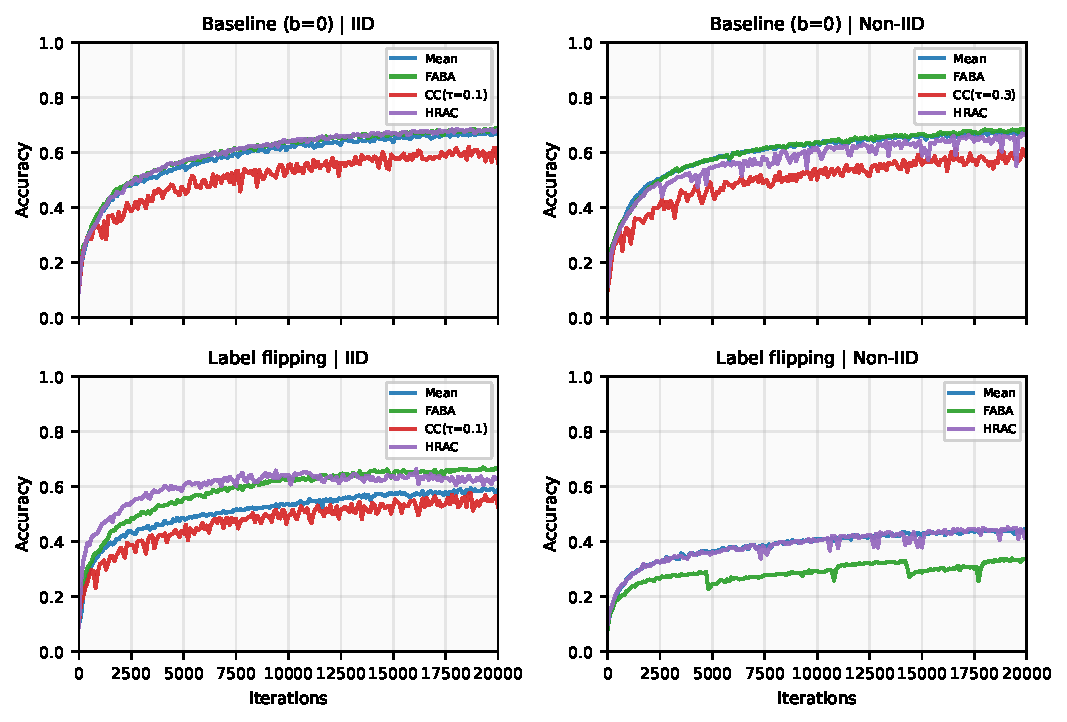
\includegraphics[width=\textwidth]{imgs/CMomentum_cifar10_b3_baseline_label_flipping}
    \caption{CIFAR-10 accuracy under benign training and label-flipping
    poisoning. The top row uses $b=0$; the label-flipping row uses $b=3$.}
    \label{fig:cifar10-baseline-label}
\end{figure}

Figure~\ref{fig:cifar10-msa-hismsa} shows attacks that manipulate update
structure or exploit temporal state. In the MSA panels, mean aggregation
degrades severely, especially under non-IID data, whereas HRAC maintains a much
higher trajectory. In the HisMSA panels, HRAC remains close to the best curves
and is particularly stable in the non-IID setting, which is consistent with the
design motivation for using client-specific history. These results show that
HRAC is most effective when the attack creates structured or persistent
deviation rather than only noisy benign variation.

\begin{figure}[p]
    \centering
    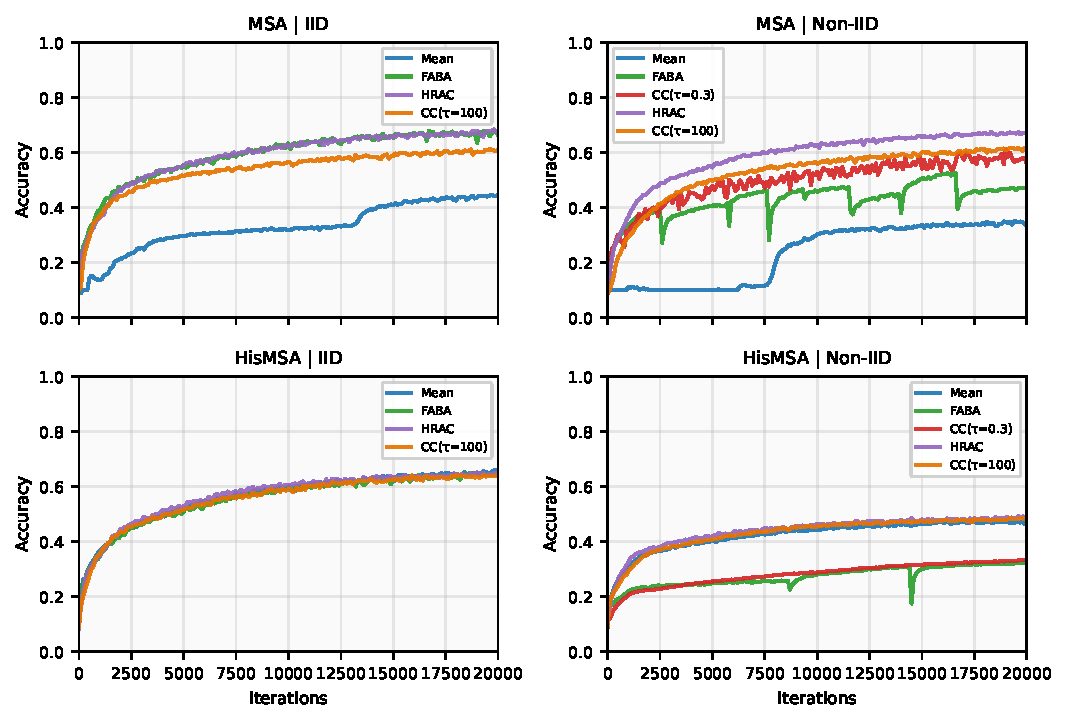
\includegraphics[width=\textwidth]{imgs/CMomentum_cifar10_b3_msa_hismsa}
    \caption{CIFAR-10 accuracy under model-shuffling (MSA) and history-aware
    model-shuffling (HisMSA) attacks with $b=3$.}
    \label{fig:cifar10-msa-hismsa}
\end{figure}

Figure~\ref{fig:cifar10-bit-alie-ipm} reports bit flipping, ALIE, and IPM. The
IID results are relatively close across several methods, but the non-IID panels
separate the defences more clearly. HRAC is consistently among the strongest
and most stable methods for non-IID ALIE and IPM. Bit flipping is more mixed in
the final-accuracy summaries: HRAC clearly suppresses the attackers in the
diagnostic plots, but FABA is higher by about five percentage points in the
non-IID $b=3$ final/best accuracy table. The centred-clipping
baseline also illustrates the limitation discussed in Chapter~\ref{ch2}: even
when used in the same baseline aggregation setting, a single centre is not a
reliable reference under the non-IID partition. Overall, the results support the
central design claim of HRAC: comparing clients against their own histories can
improve robustness to structured and history-aware attacks while preserving
benign training behaviour. At the same time, the mixed label-flipping and
bit-flipping panels show that HRAC should be treated as a robust aggregation
strategy rather than a universally dominant detector.

\begin{figure}[p]
    \centering
    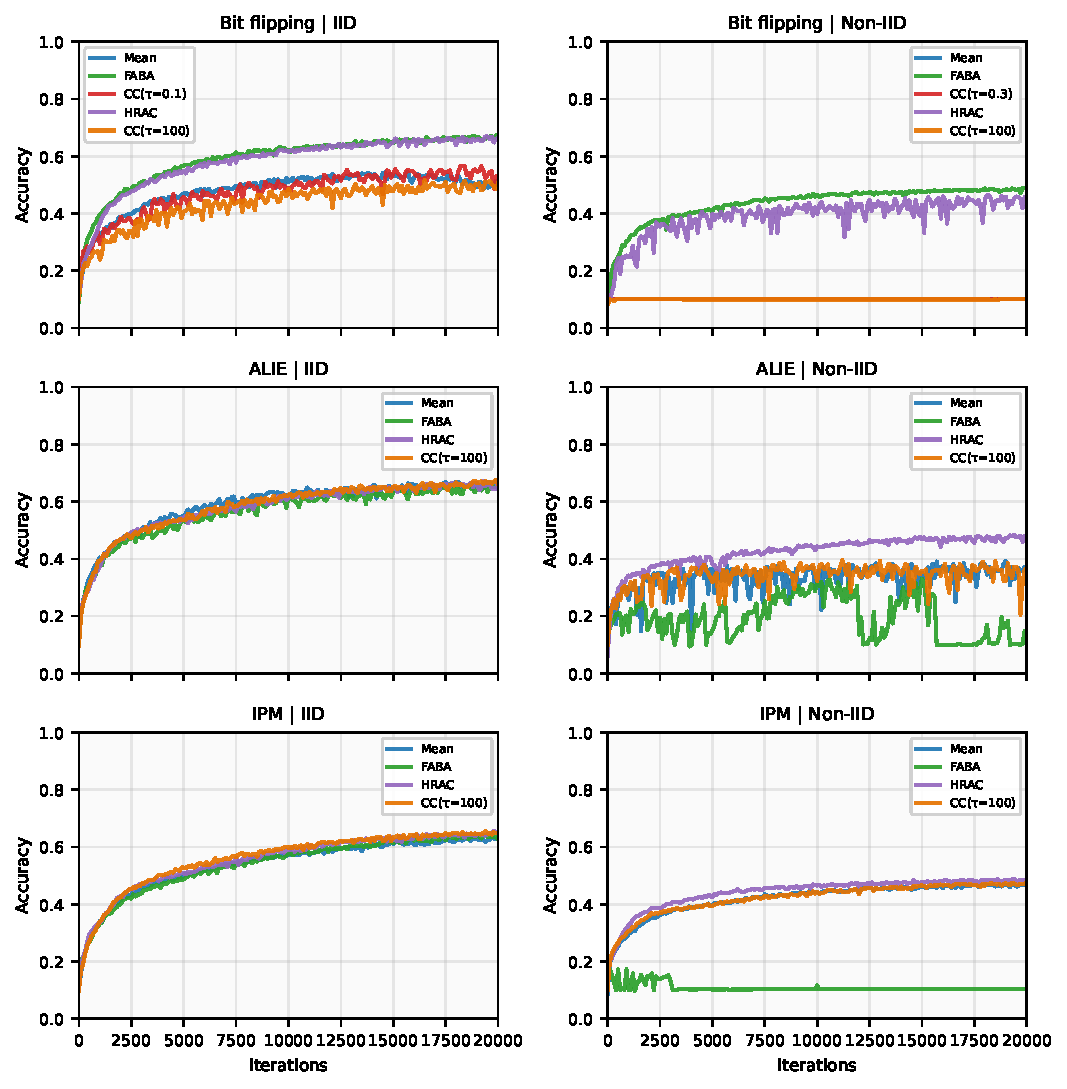
\includegraphics[width=\textwidth]{imgs/CMomentum_cifar10_b3_bit_alie_ipm}
    \caption{CIFAR-10 accuracy under bit-flipping, ALIE, and IPM attacks with
    $b=3$.}
    \label{fig:cifar10-bit-alie-ipm}
\end{figure}

Figures~\ref{fig:cifar10-b2-baseline-label}--\ref{fig:cifar10-b2-bit-alie-ipm}
repeat the same comparison with $b=2$. The lower attacker fraction reduces the
severity of several attacks, especially label flipping and ALIE, but the broad
pattern remains attack-dependent. Mean aggregation can recover in some
protocol-compliant data-poisoning settings. LFighter again remains competitive for IID label flipping but does not
resolve the non-IID label-flipping case. HRAC remains strongest in the
structured MSA setting and competitive in the remaining attacks.

\begin{figure}[p]
    \centering
    \includegraphics[width=\textwidth]{imgs/CMomentum_cifar10_b2_baseline_label_flipping}
    \caption{CIFAR-10 accuracy under benign training and label-flipping
    poisoning. The top row uses $b=0$; the label-flipping row uses $b=2$.}
    \label{fig:cifar10-b2-baseline-label}
\end{figure}

\begin{figure}[p]
    \centering
    \includegraphics[width=\textwidth]{imgs/CMomentum_cifar10_b2_msa_hismsa}
    \caption{CIFAR-10 accuracy under MSA and HisMSA attacks with $b=2$.}
    \label{fig:cifar10-b2-msa-hismsa}
\end{figure}

\begin{figure}[p]
    \centering
    \includegraphics[width=\textwidth]{imgs/CMomentum_cifar10_b2_bit_alie_ipm}
    \caption{CIFAR-10 accuracy under bit-flipping, ALIE, and IPM attacks with
    $b=2$.}
    \label{fig:cifar10-b2-bit-alie-ipm}
\end{figure}

\section{Additional Analyses}
\label{sec:additional-analyses}

Beyond the main comparison curves, the implementation was also used to isolate
which parts of HRAC are responsible for the observed behaviour. The component
study below is reported for non-IID CIFAR-10, where benign heterogeneity makes
hard filtering risky and where the main robustness claims are most relevant.
The remaining analysis focuses on what can be concluded from the available
logs, while broader sensitivity studies are treated as limitations and future
work.

\subsection{Final and Best Accuracy Summary}
\label{subsec:final-best-accuracy}

Tables~\ref{tab:final-best-accuracy} and \ref{tab:final-best-accuracy-b2}
complement the accuracy curves by reporting final-round and best observed test
accuracy. Each entry is written as ``final / best''. The best robust baseline
column is selected among FABA and CC, excluding both mean aggregation and HRAC,
so that mean aggregation remains visible as a separate reference. LFighter is
shown in the label-flipping curves but is not included in these summary tables
because cached LFighter runs are available only for label flipping, not for the
full attack suite.

\begin{table}[t]
    \centering
    \scriptsize
    \setlength{\tabcolsep}{3pt}
    \caption{Final and best CIFAR-10 test accuracy extracted from cached logs
    for the main $b=3$ attack setting. Entries are reported as final / best.}
    \label{tab:final-best-accuracy}
    \begin{tabular}{p{0.19\textwidth}p{0.13\textwidth}p{0.16\textwidth}p{0.24\textwidth}p{0.16\textwidth}}
        \hline
        \textbf{Setting} & \textbf{Partition} & \textbf{Mean} & \textbf{Best robust baseline} & \textbf{HRAC} \\
        \hline
        Baseline & IID & 0.6707 / 0.6780 & FABA: 0.6808 / 0.6887 & 0.6698 / 0.6721 \\
        Baseline & Non-IID & 0.6718 / 0.6770 & FABA: 0.6820 / 0.6857 & 0.6540 / 0.6839 \\
        Label flipping & IID & 0.5889 / 0.5951 & FABA: 0.6697 / 0.6697 & 0.6113 / 0.6152 \\
        Label flipping & Non-IID & 0.4391 / 0.4449 & CC: 0.3713 / 0.3794 & 0.4405 / 0.4429 \\
        MSA & IID & 0.4433 / 0.4464 & FABA: 0.6630 / 0.6789 & 0.6618 / 0.6618 \\
        MSA & Non-IID & 0.3369 / 0.3507 & CC: 0.5479 / 0.5626 & 0.6466 / 0.6466 \\
        HisMSA & IID & 0.6577 / 0.6593 & FABA: 0.6478 / 0.6500 & 0.6493 / 0.6732 \\
        HisMSA & Non-IID & 0.4734 / 0.4743 & CC: 0.4863 / 0.4868 & 0.4874 / 0.4912 \\
        Bit flipping & IID & 0.5006 / 0.5445 & FABA: 0.6687 / 0.6729 & 0.6685 / 0.6719 \\
        Bit flipping & Non-IID & 0.1000 / 0.1000 & FABA: 0.4875 / 0.4885 & 0.4371 / 0.4604 \\
        ALIE & IID & 0.6497 / 0.6758 & CC: 0.6607 / 0.6753 & 0.6662 / 0.6718 \\
        ALIE & Non-IID & 0.3585 / 0.3921 & CC: 0.3695 / 0.3953 & 0.4805 / 0.4846 \\
        IPM & IID & 0.6315 / 0.6348 & CC: 0.6512 / 0.6546 & 0.6459 / 0.6476 \\
        IPM & Non-IID & 0.4646 / 0.4733 & CC: 0.4736 / 0.4740 & 0.4839 / 0.4931 \\
        \hline
    \end{tabular}
\end{table}

\begin{table}[t]
    \centering
    \scriptsize
    \setlength{\tabcolsep}{3pt}
    \caption{Final and best CIFAR-10 test accuracy extracted from cached logs
    for the supplementary $b=2$ attack setting. Entries are reported as final /
    best.}
    \label{tab:final-best-accuracy-b2}
    \begin{tabular}{p{0.19\textwidth}p{0.13\textwidth}p{0.16\textwidth}p{0.24\textwidth}p{0.16\textwidth}}
        \hline
        \textbf{Setting} & \textbf{Partition} & \textbf{Mean} & \textbf{Best robust baseline} & \textbf{HRAC} \\
        \hline
        Label flipping & IID & 0.6330 / 0.6330 & FABA: 0.6638 / 0.6728 & 0.6494 / 0.6506 \\
        Label flipping & Non-IID & 0.5118 / 0.5264 & CC: 0.4461 / 0.4736 & 0.5215 / 0.5343 \\
        MSA & IID & 0.1000 / 0.1201 & FABA: 0.6544 / 0.6788 & 0.6785 / 0.6785 \\
        MSA & Non-IID & 0.1000 / 0.1000 & CC: 0.5780 / 0.5890 & 0.6628 / 0.6652 \\
        HisMSA & IID & 0.6725 / 0.6738 & FABA: 0.6615 / 0.6646 & 0.6629 / 0.6729 \\
        HisMSA & Non-IID & 0.5498 / 0.5498 & FABA: 0.4359 / 0.4363 & 0.5447 / 0.5472 \\
        Bit flipping & IID & 0.5640 / 0.5869 & FABA: 0.6642 / 0.6710 & 0.6665 / 0.6713 \\
        Bit flipping & Non-IID & 0.1000 / 0.1000 & FABA: 0.5544 / 0.5544 & 0.5227 / 0.5272 \\
        ALIE & IID & 0.6711 / 0.6711 & FABA: 0.6812 / 0.6852 & 0.6721 / 0.6721 \\
        ALIE & Non-IID & 0.5584 / 0.5618 & CC: 0.5522 / 0.5522 & 0.5571 / 0.5616 \\
        IPM & IID & 0.6601 / 0.6601 & CC: 0.6559 / 0.6667 & 0.6627 / 0.6753 \\
        IPM & Non-IID & 0.5443 / 0.5443 & CC: 0.5361 / 0.5388 & 0.5504 / 0.5565 \\
        \hline
    \end{tabular}
\end{table}

\subsection{Component Ablation Study}
\label{subsec:component-ablation}

The ablation study removes individual HRAC components while keeping the same
training setting. The tested variants remove the global median cap, remove
per-client residual clipping, remove $\nu$-based weighting, or keep only the
global cap before averaging. The goal is to check whether the observed behaviour
comes from one clipping rule or from the combination of scale control,
client-specific history, and temporal weighting.

The ALIE ablation in Figure~\ref{fig:alie-noniid-ablation} shows that the
global cap and residual clipping are not the decisive components in this run.
Both corresponding variants stay close to full HRAC
(Table~\ref{tab:alie-ablation}). In contrast, removing $\nu$ weighting causes a
large drop, and the global-cap-only variant performs similarly poorly. This
suggests that the residual-change statistic is the main useful signal against
ALIE in this experiment.

\begin{figure}[t]
    \centering
    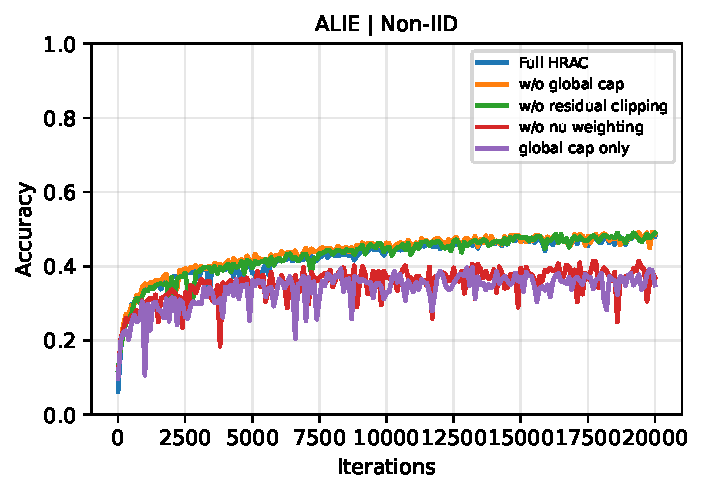
\includegraphics[width=0.82\textwidth]{imgs/CMomentum_cifar10_b3_ALIE_noniid_hrac_ablation}
    \caption{HRAC component ablation under ALIE on non-IID CIFAR-10 with
    $b=3$.}
    \label{fig:alie-noniid-ablation}
\end{figure}

\begin{table}[t]
    \centering
    \small
    \setlength{\tabcolsep}{4pt}
    \caption{Final and best test accuracy for the ALIE non-IID ablation study.}
    \label{tab:alie-ablation}
    \begin{tabular}{p{0.38\textwidth}p{0.18\textwidth}p{0.18\textwidth}p{0.18\textwidth}}
        \hline
        \textbf{Variant} & \textbf{Final} & \textbf{Best} & \textbf{Main effect} \\
        \hline
        Full HRAC & 0.4799 & 0.4843 & Reference method \\
        No global cap & 0.4863 & 0.4919 & Similar in ALIE \\
        No residual clipping & 0.4903 & 0.4903 & Similar in ALIE \\
        No $\nu$ weighting & 0.3691 & 0.4139 & Large degradation \\
        Global cap only & 0.3498 & 0.3979 & Large degradation \\
        \hline
    \end{tabular}
\end{table}

The MSA ablation in Figure~\ref{fig:msa-noniid-ablation} gives a different
pattern. Removing the global cap reduces accuracy to near chance level, while
removing residual clipping leaves a clear gap from full HRAC
(Table~\ref{tab:msa-ablation}). This indicates that MSA is controlled mainly by
explicit scale limitation, with residual clipping adding a second
history-aware constraint. The MSA ablation values come from a separate
controlled ablation cache rather than the main comparison cache used in
Table~\ref{tab:final-best-accuracy}, so the full-HRAC reference value is not
identical to the MSA entry in the main summary table.

\begin{figure}[t]
    \centering
    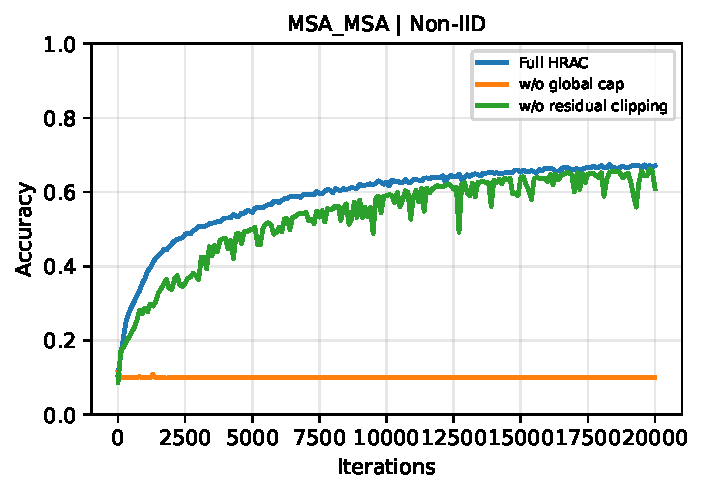
\includegraphics[width=0.82\textwidth]{imgs/CMomentum_cifar10_b3_MSA_MSA_noniid_hrac_ablation}
    \caption{HRAC component ablation under MSA on non-IID CIFAR-10 with
    $b=3$.}
    \label{fig:msa-noniid-ablation}
\end{figure}

\begin{table}[t]
    \centering
    \small
    \setlength{\tabcolsep}{4pt}
    \caption{Final and best test accuracy for the MSA non-IID ablation study.
    These controlled ablation runs use a separate cache from the main comparison
    in Table~\ref{tab:final-best-accuracy}; therefore the full-HRAC reference
    value differs from the main-table HRAC value.}
    \label{tab:msa-ablation}
    \begin{tabular}{p{0.42\textwidth}p{0.20\textwidth}p{0.20\textwidth}}
        \hline
        \textbf{Variant} & \textbf{Final} & \textbf{Best} \\
        \hline
        Full HRAC & 0.6713 & 0.6743 \\
        No global cap & 0.1000 & 0.1163 \\
        No residual clipping & 0.6099 & 0.6615 \\
        \hline
    \end{tabular}
\end{table}

Overall, the ablations show that HRAC's components matter in different ways for
different attacks. Temporal weighting is most useful for ALIE, while the global
cap is essential for MSA and residual clipping gives additional protection. This
supports keeping the three mechanisms together rather than treating HRAC as a
single clipping heuristic.

\subsection{Diagnostic Analysis}
\label{subsec:diagnostic-analysis}

The HRAC logs also allow the accuracy results to be connected to the internal
statistics used by HRAC. During training, the implementation records
per-round residual thresholds $\tau_i$, residual scale statistics $\mu_i$,
residual-change statistics $\nu_i$, normalised client weights, pre- and
post-clipping norms, and bottom-weight summaries for controlled simulation
runs.

The diagnostic plots are treated as supporting analysis rather than as the
primary evidence for HRAC. The left panel tracks the average residual-change
statistic $\nu_i$ for benign and Byzantine clients, the middle panel shows their
normalised aggregation weights, and the right panel counts how many Byzantine
clients appear among the three lowest-weighted clients. The main empirical
claims in this chapter therefore rest on the accuracy curves, final/best
accuracy summaries, and component ablations, while diagnostics are used to
interpret those results.

Across most attacks, these diagnostics show the intended behaviour. Once the
weighting stage becomes active, Byzantine clients tend to have larger
residual-change statistics, receive lower average weights, and appear
frequently in the bottom-weight set. This pattern is visible for bit flipping,
ALIE, IPM, HisMSA, and IID label flipping. It suggests that the weighting rule
is often suppressing the clients that generate abnormal residual dynamics.

The weaker cases are also informative. For MSA, strong accuracy does not always
come with clean attacker identification in the weight diagnostics. This is
consistent with the ablation result, where the global cap is the decisive
component and limits the effect of shuffled or amplified updates even when the
weights are not a reliable detector. For label flipping, the IID case still
shows clear attacker down-weighting, but the non-IID case is harder. Benign
label-skew already creates client-specific residual variation, so poisoned and
benign $\nu_i$ trajectories overlap more strongly and the bottom-weight summary
captures the attackers less consistently. This is why protocol-compliant label
poisoning becomes more difficult when it is combined with heterogeneous data.

\begin{figure}[p]
    \centering
    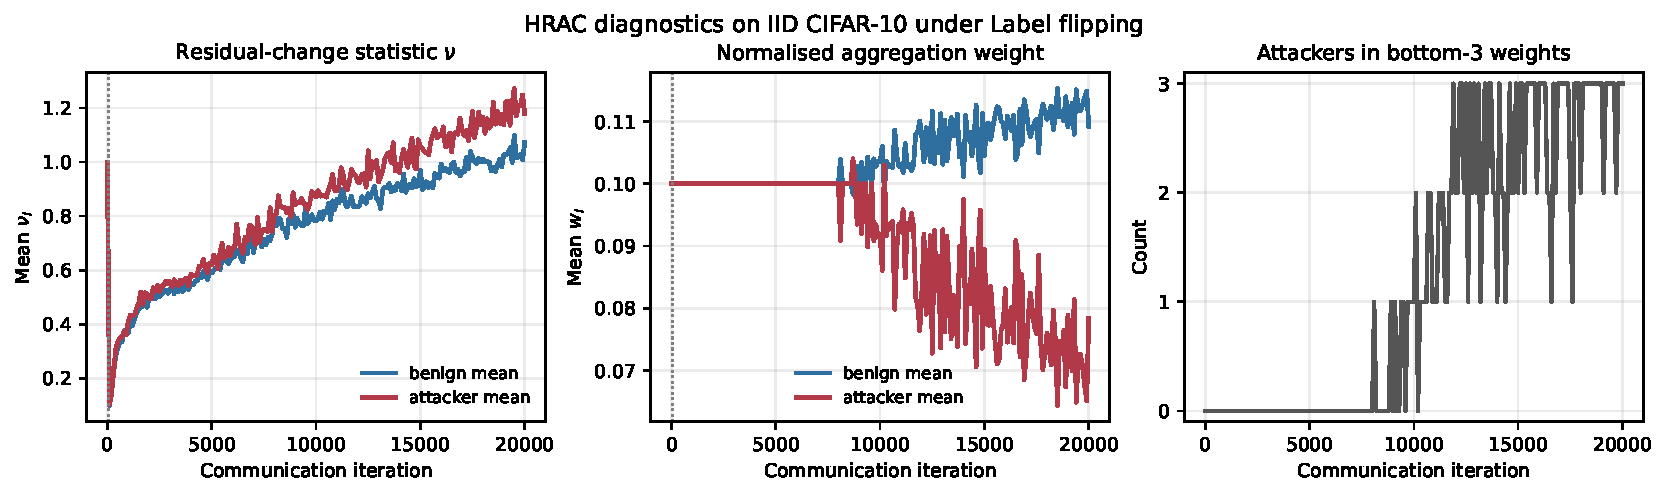
\includegraphics[width=\textwidth]{imgs/hrac_diagnostics_all_attacks/HRAC_diagnostics_label_flipping_iid}
    \vspace{0.5em}
    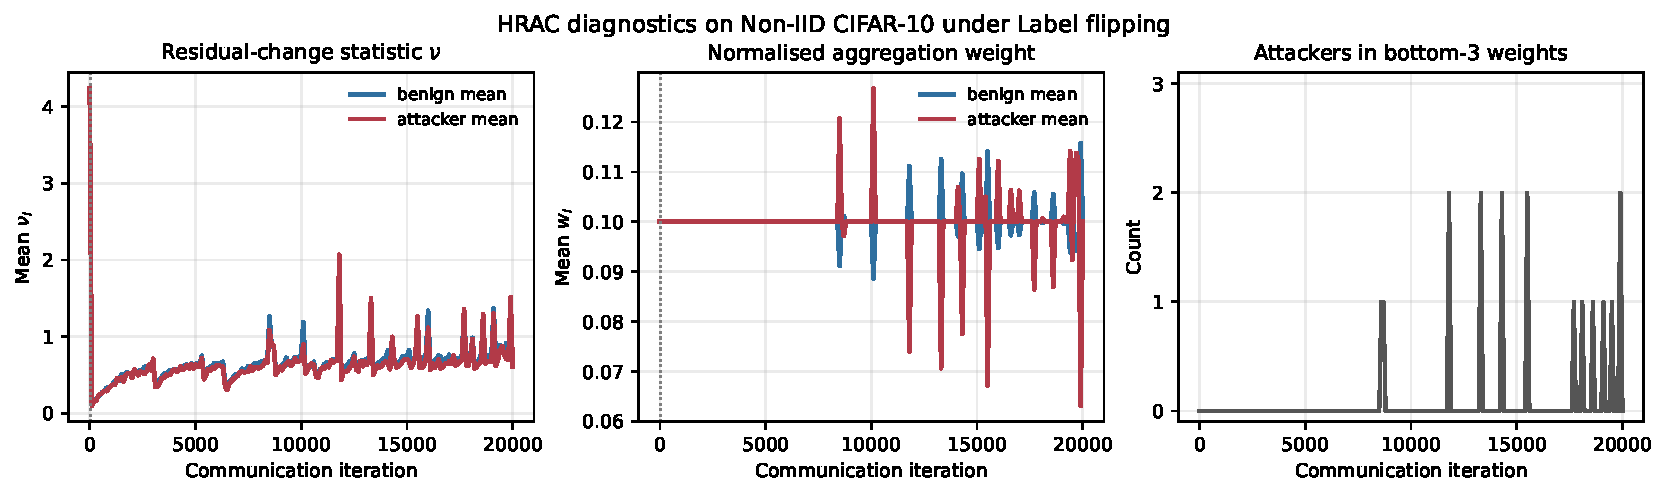
\includegraphics[width=\textwidth]{imgs/hrac_diagnostics_all_attacks/HRAC_diagnostics_label_flipping_noniid}
    \caption{HRAC diagnostics under label-flipping attacks for IID and non-IID
    CIFAR-10.}
    \label{fig:diag-label-flipping}
\end{figure}

\begin{figure}[p]
    \centering
    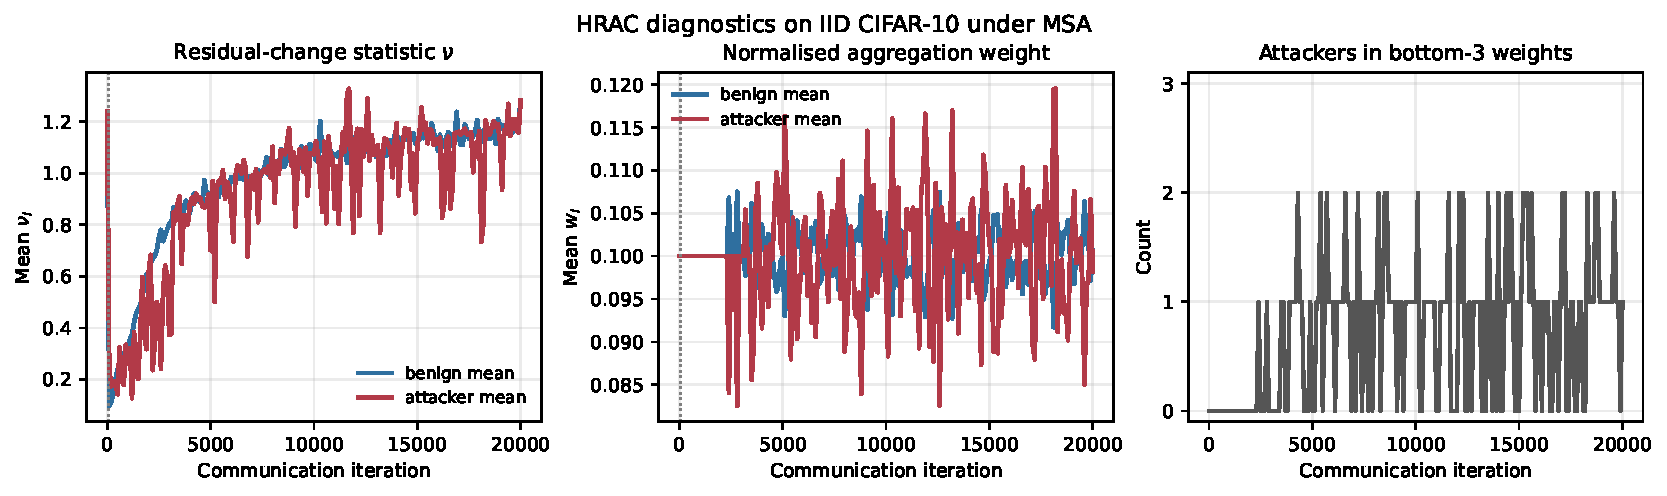
\includegraphics[width=\textwidth]{imgs/hrac_diagnostics_all_attacks/HRAC_diagnostics_MSA_iid}
    \vspace{0.5em}
    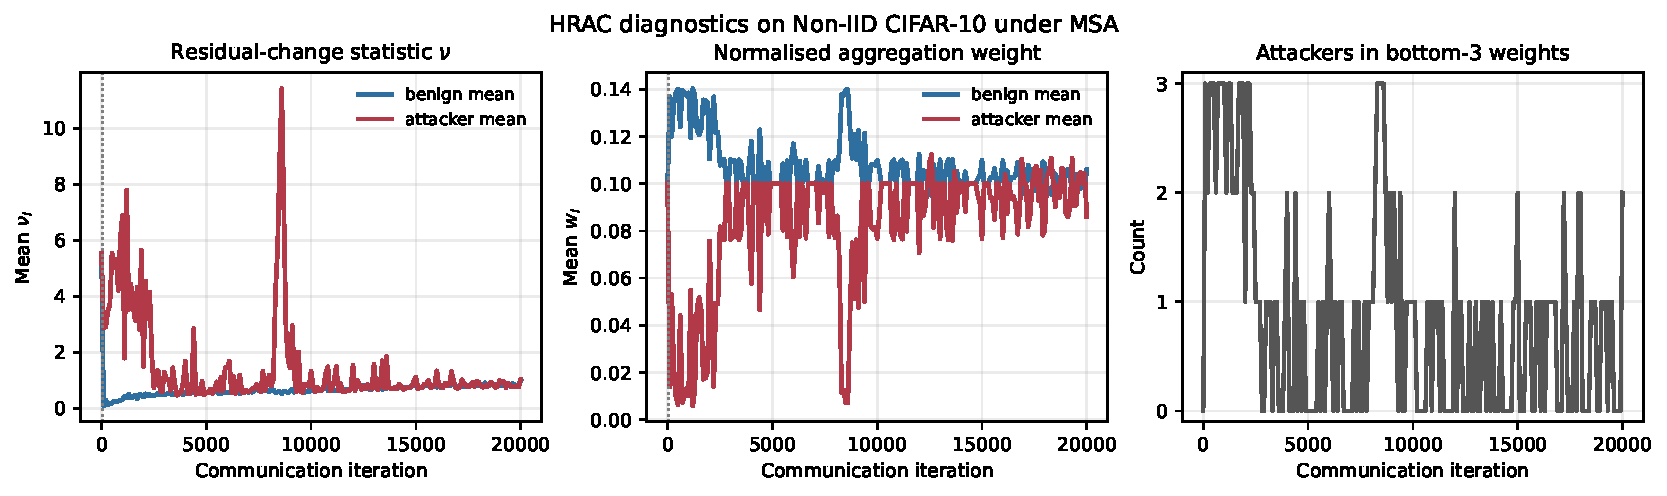
\includegraphics[width=\textwidth]{imgs/hrac_diagnostics_all_attacks/HRAC_diagnostics_MSA_noniid}
    \caption{HRAC diagnostics under MSA attacks for IID and non-IID CIFAR-10.}
    \label{fig:diag-msa}
\end{figure}

\begin{figure}[p]
    \centering
    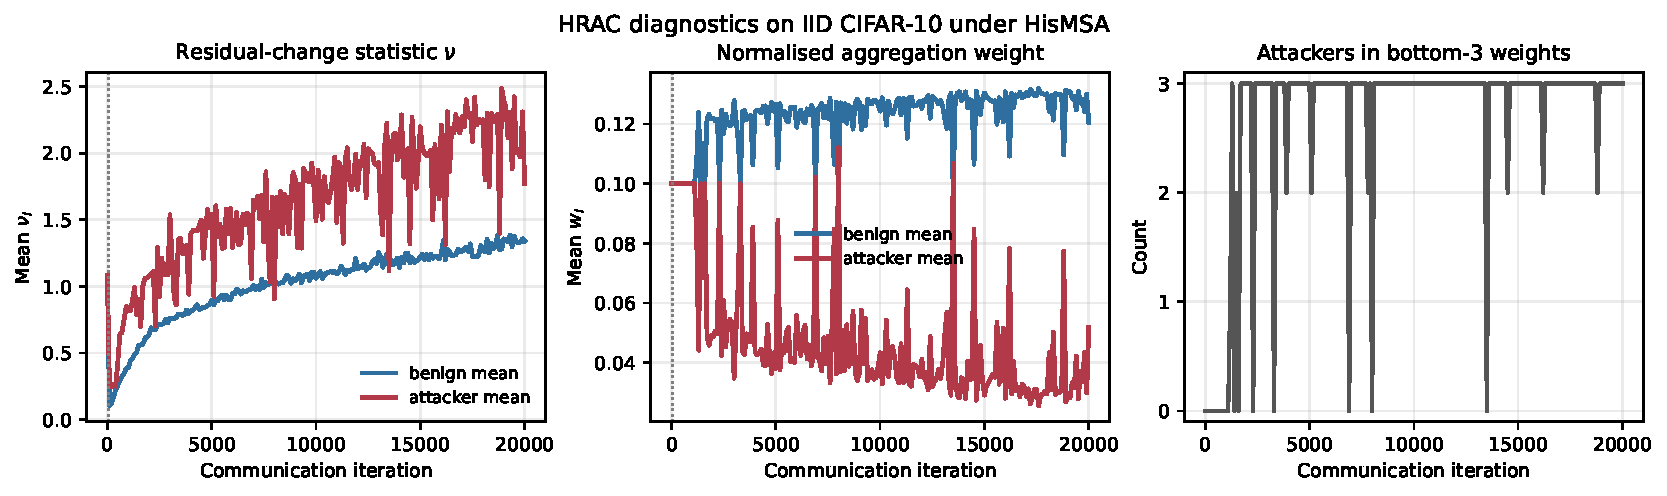
\includegraphics[width=\textwidth]{imgs/hrac_diagnostics_all_attacks/HRAC_diagnostics_HisMSA_iid}
    \vspace{0.5em}
    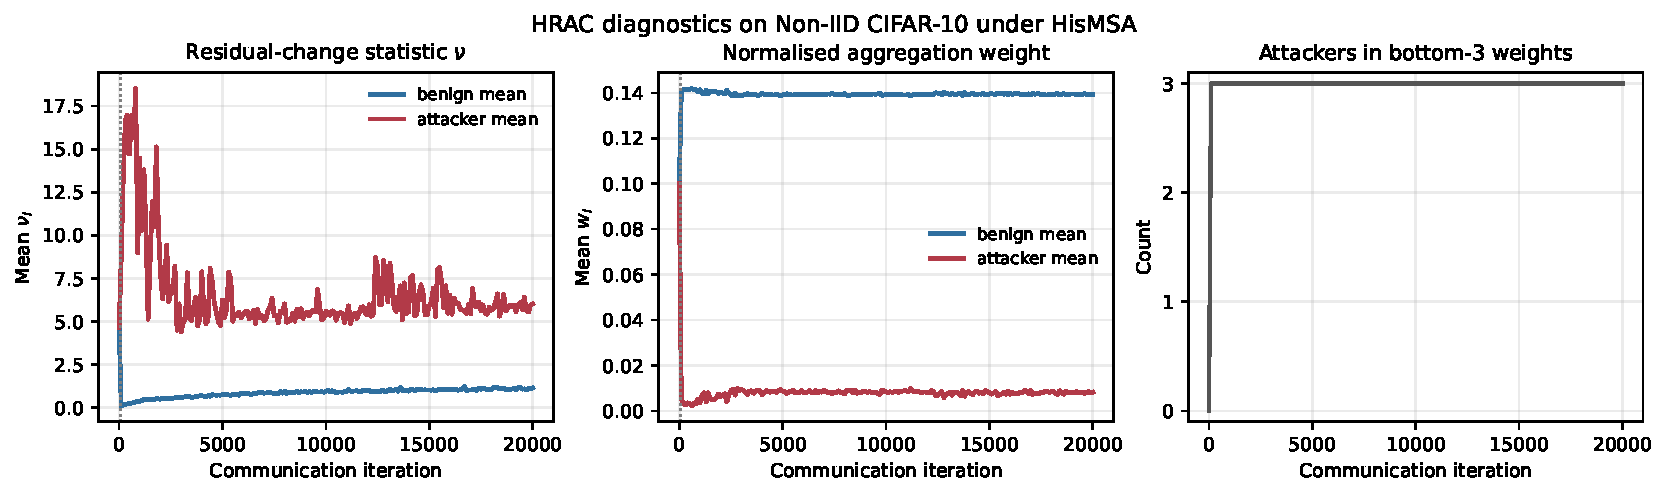
\includegraphics[width=\textwidth]{imgs/hrac_diagnostics_all_attacks/HRAC_diagnostics_HisMSA_noniid}
    \caption{HRAC diagnostics under HisMSA attacks for IID and non-IID
    CIFAR-10.}
    \label{fig:diag-hismsa}
\end{figure}

\begin{figure}[p]
    \centering
    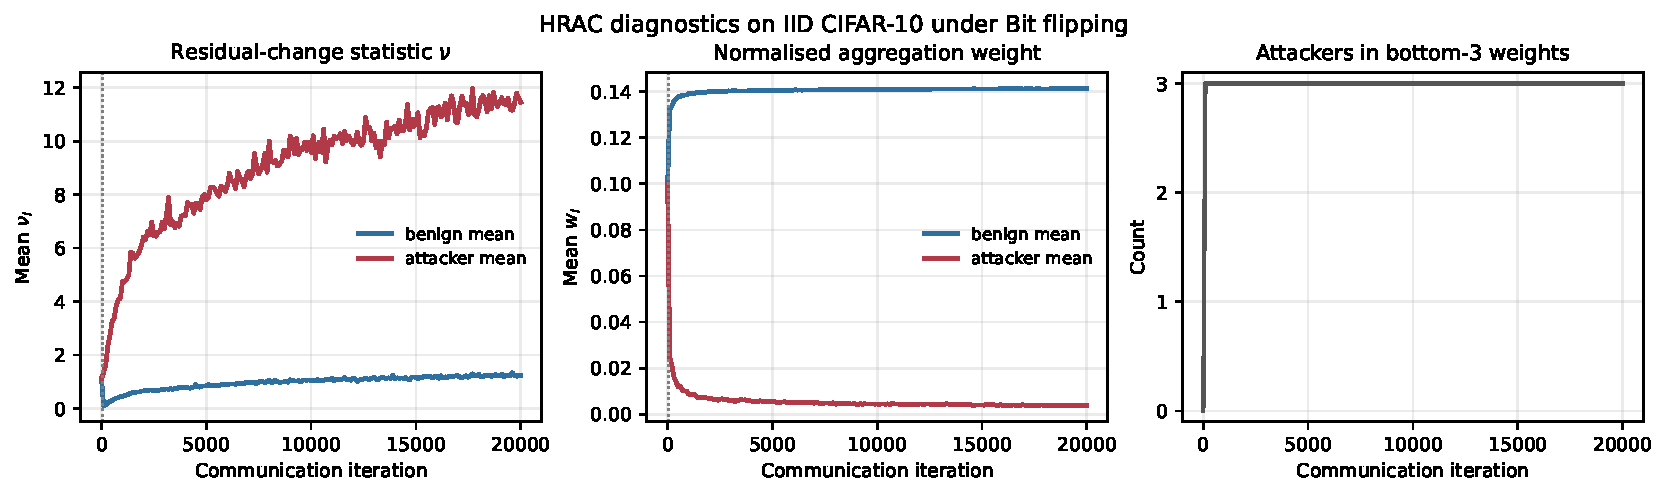
\includegraphics[width=\textwidth]{imgs/hrac_diagnostics_all_attacks/HRAC_diagnostics_bit_flipping_iid}
    \vspace{0.5em}
    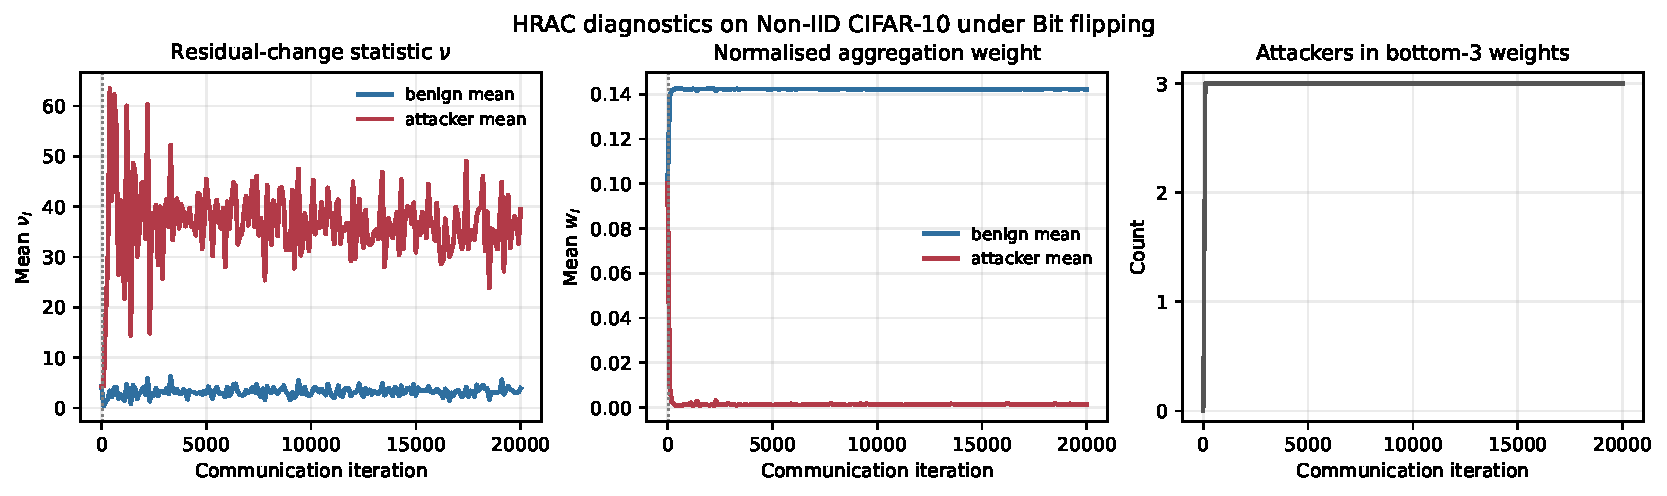
\includegraphics[width=\textwidth]{imgs/hrac_diagnostics_all_attacks/HRAC_diagnostics_bit_flipping_noniid}
    \caption{HRAC diagnostics under bit-flipping attacks for IID and non-IID
    CIFAR-10.}
    \label{fig:diag-bit-flipping}
\end{figure}

\begin{figure}[p]
    \centering
    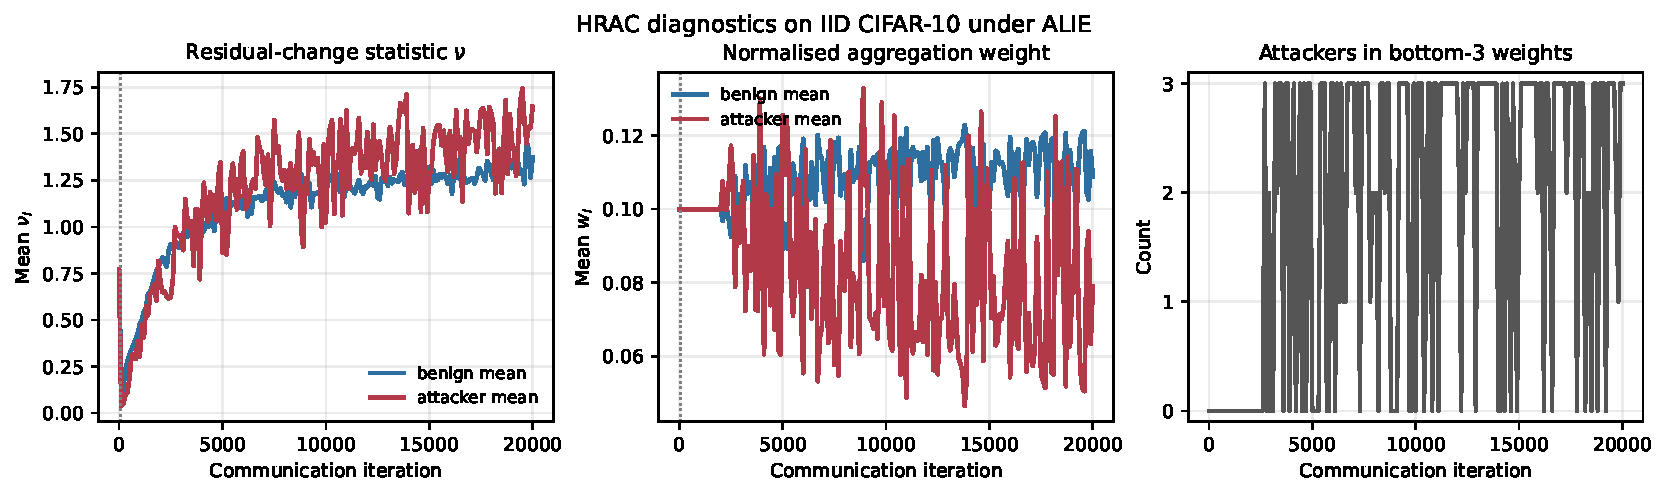
\includegraphics[width=\textwidth]{imgs/hrac_diagnostics_all_attacks/HRAC_diagnostics_ALIE_iid}
    \vspace{0.5em}
    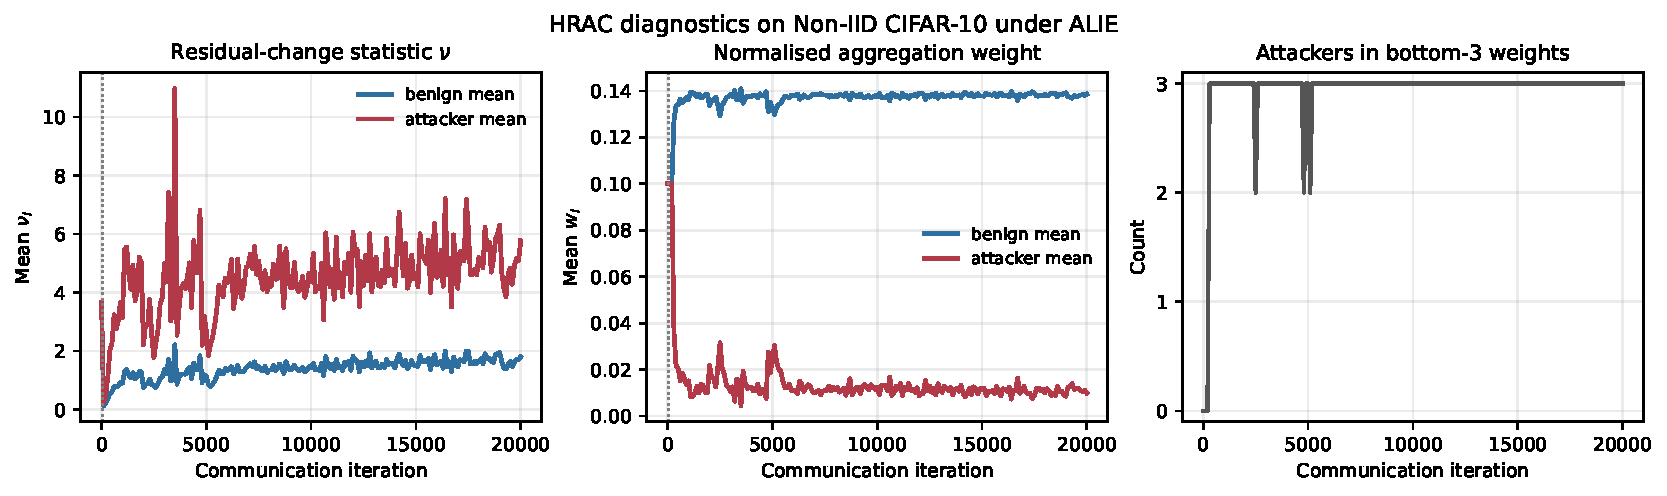
\includegraphics[width=\textwidth]{imgs/hrac_diagnostics_all_attacks/HRAC_diagnostics_ALIE_noniid}
    \caption{HRAC diagnostics under ALIE attacks for IID and non-IID CIFAR-10.}
    \label{fig:diag-alie}
\end{figure}

\begin{figure}[p]
    \centering
    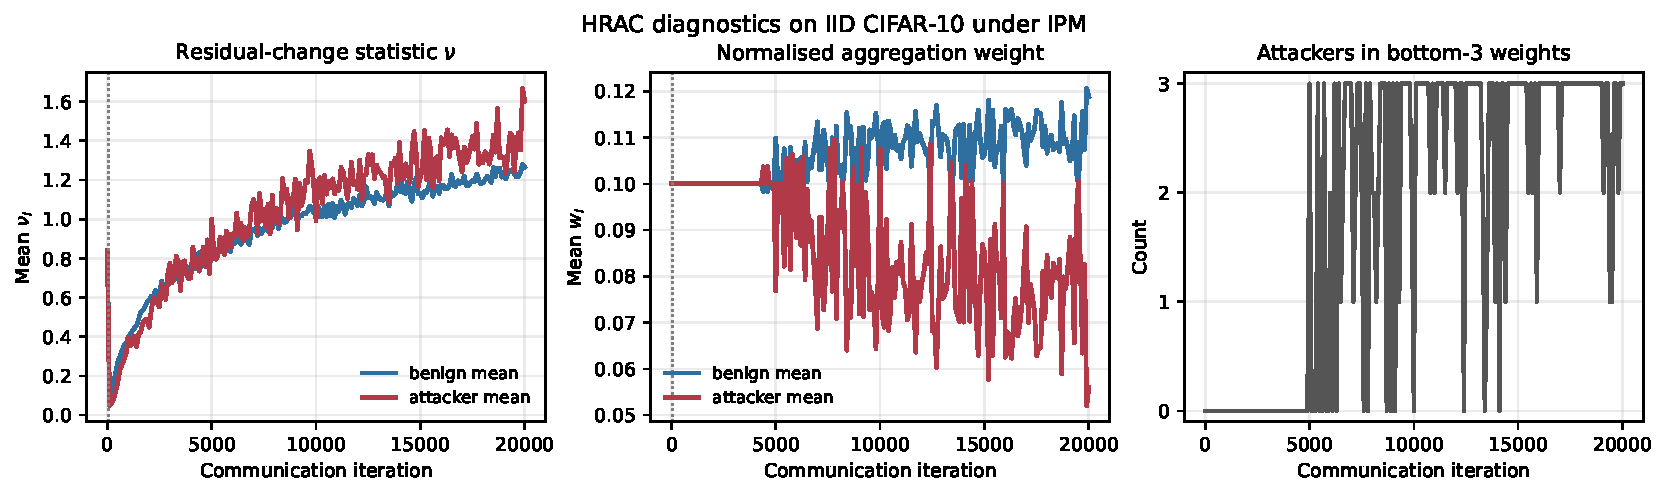
\includegraphics[width=\textwidth]{imgs/hrac_diagnostics_all_attacks/HRAC_diagnostics_IPM_iid}
    \vspace{0.5em}
    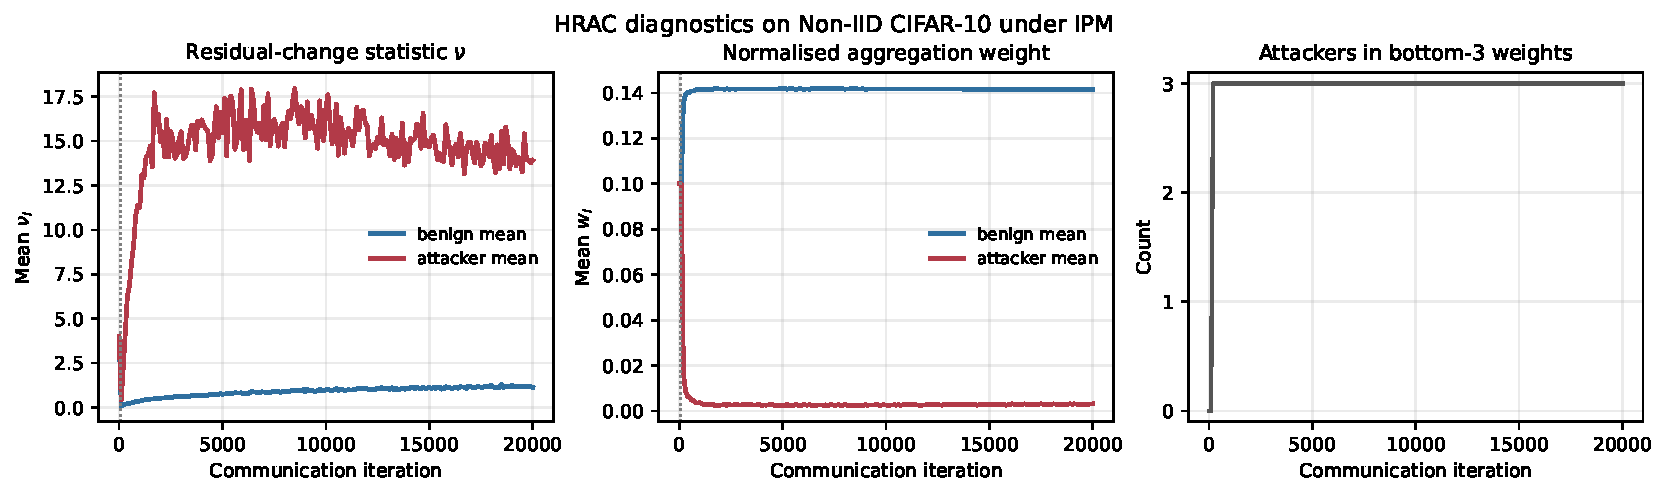
\includegraphics[width=\textwidth]{imgs/hrac_diagnostics_all_attacks/HRAC_diagnostics_IPM_noniid}
    \caption{HRAC diagnostics under IPM attacks for IID and non-IID CIFAR-10.}
    \label{fig:diag-ipm}
\end{figure}

\section{Discussion and Limitations}
\label{sec:discussion-limitations}

The experimental results match the trade-off stated in the abstract. Mean
aggregation can remain competitive for protocol-compliant poisoning under
heterogeneous data, but it is not reliable under stronger model-poisoning
attacks. Some robust baselines are
strong in particular cases, but their relative ranking changes with the attack
and partition. HRAC is most useful when malicious behaviour appears as
structured or persistent deviation, as in MSA, HisMSA, non-IID ALIE, and
non-IID IPM.

The mixed label-flipping and bit-flipping results are therefore part of the
claim rather than an exception to it. Under IID label flipping, HRAC performs
well because poisoned clients stand out more clearly from a relatively aligned
benign population. The diagnostic plot supports this because attacker weights
decline over training, and the bottom-weight set increasingly contains the
Byzantine clients. Under non-IID label flipping, the difficulty comes from the
interaction between the attack and the data partition rather than from label
flipping alone. Benign label-skew already produces client-specific residual
variation, so the $\nu$ trajectories of benign and poisoned clients overlap
much more, and the bottom-weight summary captures the attackers less
consistently. LFighter follows a similar pattern in the available
label-flipping runs, where it is strong under IID data but weaker under the
non-IID partition. Bit flipping is different: in the diagnostic plots, the
attacker $\nu$ values separate strongly from the benign clients, the attacker
weights are pushed close to zero, and the bottom-weight summary consistently
contains the Byzantine clients. HRAC should therefore be read as a balanced
robust aggregation strategy, not as a specialised label-poisoning defence.

The main limitations are the fixed HRAC hyperparameter setting and the
restricted experiment grid. The current cached results use CIFAR-10, \(N=10\)
clients, seed 100, \(b=2\) and \(b=3\) attack settings, and one label class per
client for the non-IID partition. The attack parameters are also fixed in the
reported runs, for example IPM uses \(\epsilon=0.1\) and MSA/HisMSA use shuffle
probability 1.0 with scaling range \((0.1,10.0)\). A stronger empirical study
would rerun the same comparison across multiple seeds, datasets, client counts,
attacker fractions, label-skew severities, and attack strengths.

% \input{chapters/chapter5 }
% \doublespacing % Do not change - required

\chapter{Project Plan}
\label{chPlan}

%%%%%%%%%%%%%%%%%%%%%%%%%%%%%%%%%%%%%%%
% IMPORTANT
\begin{spacing}{1} %THESE FOUR
\minitoc % LINES MUST APPEAR IN
\end{spacing} % EVERY
\thesisspacing % CHAPTER
% COPY THEM IN ANY NEW CHAPTER
%%%%%%%%%%%%%%%%%%%%%%%%%%%%%%%%%%%%%%%

\section{Overview}

The project develops and evaluates robust aggregation methods for federated learning under the Byzantine threat model, with a focus on non-IID client heterogeneity and history-aware attacks. Work is organised into a small number of work packages (WPs) with clear deliverables and review points.

\section{Work Packages}

\begin{itemize}
    \item \textbf{WP1: Background and Specification (Weeks 1--2).}
    Review robust aggregation and history-aware attacks; define threat model, datasets, baselines, and success criteria. 
    \textit{Deliverables:} project specification, literature summary, experimental protocol.

    \item \textbf{WP2: Implementation of Defences (Weeks 2--5).}
    Implement HSM-Adaptive in the federated training pipeline, including logging/diagnostics and modular support for baselines.
    \textit{Deliverables:} working codebase, unit/sanity checks, reproducible configs.

    \item \textbf{WP3: Attack Models and Benchmarks (Weeks 4--6).}
    Implement and validate attack models (e.g., label flipping, scaling, MSA/shuffle, history-aware variants) under IID and non-IID partitions.
    \textit{Deliverables:} verified attack suite, benchmark scripts, plotting utilities.

    \item \textbf{WP4: Experimental Evaluation (Weeks 6--9).}
    Run controlled experiments, tune parameters conservatively, and conduct ablations to assess component contributions.
    \textit{Deliverables:} result tables/figures, ablation findings, robustness--utility analysis.

    \item \textbf{WP5: Dissertation Writing and Refinement (Weeks 8--11).}
    Write chapters (method, implementation, experiments, results), incorporate supervisor feedback, and finalise presentation quality.
    \textit{Deliverables:} complete draft, revised final submission, reproducibility appendix.
\end{itemize}

\section{Milestones and Risk Management}

Key milestones are (i) a complete baseline+attack pipeline, (ii) a stable HSM-Adaptive implementation with diagnostics, and (iii) a complete evaluation set with ablations. Primary risks include unstable training under strong attacks, sensitivity to hyper-parameters, and time overruns due to repeated experiments. Mitigations include fixed seeds, staged experiments (small-scale first), incremental logging, and prioritising a minimal set of decisive comparisons before optional extensions.


\doublespacing % Do not change - required

\chapter{Professional Issues and Project Management}
\label{chLast}

%%%%%%%%%%%%%%%%%%%%%%%%%%%%%%%%%%%%%%%
% IMPORTANT
\begin{spacing}{1}
\minitoc
\end{spacing}
\thesisspacing
%%%%%%%%%%%%%%%%%%%%%%%%%%%%%%%%%%%%%%%

\section{Project Plan}

The project was organised into work packages (WPs) covering literature review, baseline reproduction, attack integration, HRAC implementation, experimental evaluation, and final write-up. Early effort was concentrated on establishing a reliable experimental pipeline, including datasets, training loops, attack baselines, logging, and plotting, so that later conclusions would not be limited by tooling or reproducibility issues.

Progress was managed through weekly milestones defined by measurable outcomes rather than only dates. Core milestones included reproducing a stable benign baseline, validating each attack setting, integrating HRAC into the common training loop, and producing result tables, ablations, and diagnostic logs. When outcomes deviated from expectations, the plan was revised by updating estimates and re-prioritising tasks, particularly during phases where debugging and experimental variance dominated progress.

Risk management focused on training instability under non-IID partitions, hyperparameter sensitivity, and limited feedback cycles. Mitigations included staged evaluation from IID to non-IID settings, fixed configurations for main comparisons, and early production of intermediate results. A contingency path was also defined: if HRAC did not consistently outperform strong baselines, the project would still deliver a defensible contribution through ablation studies, failure-mode analysis, and clear reporting of limitations.

\section{Evaluation Plan}

The evaluation was structured around three questions: whether HRAC preserves benign utility, whether it improves robustness under Byzantine behaviour without oracle attacker labels, and whether its logged residual and weighting signals help explain the observed behaviour.

Results are reported across IID and non-IID partitions, with the main CIFAR-10 attack settings using $b=3$ malicious clients out of $N=10$. The attack set includes protocol-compliant label flipping, structural model manipulation, history-aware manipulation, and variance- or direction-based attacks. All methods are evaluated under matched training settings, and the limited seed and attacker-fraction coverage is reported explicitly in Chapter~\ref{ch:experiments-results}.

Success is measured primarily through test-accuracy trajectories, final and best accuracy, and component ablations. Diagnostic logs, including residual thresholds, $\mu/\nu$ histories, normalised weights, and attacker-aware summaries, are used to support interpretation rather than to define success alone.

Component-level justification is provided through ablation studies that disable individual HRAC mechanisms while keeping the surrounding pipeline fixed. Reproducibility is supported by cached records, logged configurations, and standardised plots and tables across methods. Additional seeds, datasets, and attacker fractions remain important extensions beyond the current scope.

\section{Legal and Ethical Matters}

This project investigates robustness in federated/distributed learning under the Byzantine threat model. The work is conducted as a research and engineering study using established open-source software and publicly available benchmark datasets for academic evaluation. It does not involve deployment in a live operational environment or the collection of new personal data.

\textbf{Legal considerations.}
The implementation relies on third-party libraries and datasets distributed under open licences. Their licence terms and attribution requirements are respected through appropriate citation and acknowledgement in the dissertation and accompanying codebase. From a data protection perspective, experiments are performed on standard public datasets rather than personal or sensitive user records. The project nevertheless recognises that, in real-world federated learning deployments, model updates may carry information that could be considered sensitive. Any future deployment would therefore require suitable governance and technical controls (e.g., access control, secure aggregation, and procedures consistent with applicable data protection regulation such as GDPR).

\smallskip

\textbf{Ethical considerations.}
The project includes adversarial behaviours to evaluate robustness systematically; the intent is defensive and scientific rather than enabling misuse. Ethical risks are mitigated by focusing on aggregate results and interpretable diagnostic statistics, and by avoiding unnecessary dissemination of operational misuse guidance. The work also considers the ethical risk of unfairly penalising benign clients under non-IID data heterogeneity. To reduce such harm, HRAC compares clients mainly with their own histories and applies continuous suppression rather than rigid exclusion.

\section{Impact}

The main environmental impact of this project comes from compute used for repeated training runs (attacks, baselines, and ablations). This is limited by keeping experiments tightly scoped, reusing standard benchmarks, and logging results carefully to avoid unnecessary reruns. The defence itself is lightweight on the server side because it uses vector norm operations and per-client EMA states, so it does not add substantial overhead per round.

Societally, more robust federated learning can make privacy-preserving systems more reliable in areas such as edge sensing, healthcare, and industrial monitoring. The main risks are increased compute in large deployments and the possibility that benign but highly non-IID clients are down-weighted over time. These are reduced by using client-specific histories, soft weighting rather than hard exclusion, and participation diagnostics to catch unwanted behaviour early.

\section{EDI}

Equality, Diversity, and Inclusion considerations are reflected in the project's emphasis on heterogeneous client behaviour. Non-IID data is treated as a first-class condition, which in real deployments may correspond to diversity in users, devices, environments, and usage patterns. Robust aggregation methods can unintentionally disadvantage minority or atypical yet benign clients if they rely on tight clustering assumptions. HRAC mitigates this risk by using each client's historical residual behaviour as the main reference, aiming to remain tolerant to legitimate variability while still resisting adversarial manipulation.

In addition, the project maintains interpretable diagnostics (per-client residual statistics and weighting statistics) to support auditing and to identify systematic patterns of misclassification that could disproportionately affect particular client populations. These practices contribute to a more transparent and accountable engineering process for systems intended to operate across diverse participants.

\section{Quality Management}

Quality was maintained using standard software and experimental practice. All code and configurations were tracked with version control to support traceability and reproducibility. Experiments were run with consistent settings (including fixed random seeds where appropriate) and key metrics were logged in a structured way (e.g., accuracy, $\tau/\mu/\nu$ statistics, aggregation weights, and attacker-aware diagnostics).

Basic validation checks were built into the pipeline, including numerical stability safeguards and sanity checks on intermediate values (such as weight non-negativity and normalisation). We also ran benign-condition regression tests to ensure the defence does not degrade normal training, and used baseline comparisons and ablations to verify the effect of each component.

\section{Safety Plan}

This project is a software-only study on public benchmark datasets and does not involve laboratory
equipment, hardware prototyping, human participants, or hazardous materials. Therefore, there are no
significant physical safety risks.

The main remaining risks are minimal and relate to good computing practice: ensuring code and results are
stored securely, avoiding any sensitive or personally identifiable data in datasets/logs, and documenting
the experimental setup to prevent misuse or misinterpretation of results. Any future deployment in
safety-critical domains would require a separate, domain-specific safety assessment.


% You can change the title of the conclusions by changing the text between { }
\conclusions{Conclusions and future directions} % Do not remove - required
% EDIT THE CONTENT OF THE FILE
% Conclusions.tex
% You can find it under the folder 
% "chapters" on the left column

% APPENDICES ARE OPTIONAL
% COMMENT OUT BOTH LINES BELOW TO REMOVE THEM
% ADD CHAPTERS TO ADD MULTIPLE APPENDICES
\appendix
\doublespacing % Do not change - required

\chapter{Convergence Analysis of HRAC}
\label{app:convergence-analysis}

\thesisspacing % Do not change - required

This appendix gives the conditional convergence argument supporting the brief
statement in Chapter~\ref{ch:method-implementation}. The proof treats HRAC as a
robust aggregation rule with bounded clipping distortion, bounded history-state
growth, and bounded residual Byzantine weight mass, then inserts the resulting
aggregation error into a standard smooth non-convex descent argument. It should
be read as a bounded-influence stability analysis under stated assumptions, not
as a proof that HRAC identifies Byzantine clients in all settings.
\section{Introduction}

The goal is to separate the proof into two parts. Rather than proving the code
line by line, HRAC is abstracted as a robust aggregation rule and analysed as
follows:

\begin{enumerate}[label=\arabic*.]
    \item show that the HRAC aggregate remains close to the ideal honest
    conditional centre;
    \item show that such an aggregation error can be absorbed into the descent
    analysis of smooth non-convex optimisation.
\end{enumerate}

For the adaptive statistics, the main theorem-level target is not universal
pointwise ordering between Byzantine and honest clients at every late-stage
round. Instead, the primary claim is the weaker and empirically better-matched
one: Byzantine clients exhibit a larger late-stage group-mean \(\nu\)-band,
which induces stronger penalty pressure and smaller weights once the activation
threshold becomes active. In particular, the intended mechanism is not that
honest statistics vanish while Byzantine statistics remain nonzero. Rather,
both groups may stay in positive late-stage bands, while Byzantine clients are
typically elevated relative to the honest population. Pointwise separation is
kept as a stronger sufficient refinement.

The clipping argument is stated at the level needed for this dissertation. To
make the global cap compatible with the clipped-moment lemma of Sadiev
et al.~\cite{sadiev2023highprob}, HRAC uses a lagged history-EMA median scale
as its global clipping radius. Thus the global threshold is
\(\F_t\)-measurable at round \(t\), just like the residual threshold determined
by the HRAC history state. The price of this proof route is a strong bounded
honest-update assumption, so the result certifies bounded-influence behaviour
rather than a full distribution-free FL guarantee.

\section{Problem Setup}

Let \(x_t \in \R^d\) denote the global model at round \(t\).
Suppose there are \(N\) participating clients, partitioned into an honest set
\(\HH\) and a Byzantine set \(\BB\), with
\[
    |\HH| = H, \qquad |\BB| = B, \qquad N = H + B.
\]

At round \(t\), the server receives client messages
\[
    \{\Delta_i^t\}_{i=1}^N \subset \R^d,
\]
where \(\Delta_i^t\) denotes a gradient-like descent direction, as in
Chapters~\ref{ch2} and~\ref{ch:method-implementation},
and performs the global update
\begin{equation}
    x_{t+1} = x_t - \eta_t g_t,
    \label{eq:server_update}
\end{equation}
where \(g_t\) is the aggregate produced by HRAC.

The optimization proof below uses the conditional honest centre as the
reference object, because the clipped-moment lemma of
Sadiev et al.~\cite[Lemma~5.1]{sadiev2023highprob} is stated conditionally on
\(\F_t\). For honest clients, define
\begin{equation}
    m_i^t:=\E[\Delta_i^t\mid\F_t],
    \qquad i\in\HH,
    \label{eq:honest_conditional_centre}
\end{equation}
and the average honest conditional centre
\begin{equation}
    \bar m_{\HH}^t
    :=
    \frac1H\sum_{i\in\HH}m_i^t.
    \label{eq:honest_centre_average}
\end{equation}

The objective is to minimise a possibly non-convex function
\[
    f : \R^d \to \R.
\]

\section{HRAC Aggregation Rule}

HRAC operates in three stages.

\subsection{Global norm clipping}

Define the current round median norm
\begin{equation}
    M_t := \med_{1\le j\le N}\norm{\Delta_j^t}.
    \label{eq:round_median_norm}
\end{equation}
HRAC maintains a history-EMA global scale
\begin{equation}
    s_{t+1}
    =
    \rho_gs_t+(1-\rho_g)M_t,
    \qquad 0<\rho_g<1,
    \label{eq:global_scale_ema}
\end{equation}
and uses the predictable global clipping cap with a fixed positive floor
\begin{equation}
    B_t := c_g\max\{s_t,s_{\min}\},
    \qquad c_g\ge1,\quad s_{\min}>0.
    \label{eq:global_cap}
\end{equation}
Thus \(B_t\in\F_t\): the current round median \(M_t\) updates the next round's
radius but is not used to clip the current round's updates. The globally
clipped update is
\begin{equation}
    \bar{\Delta}_i^t
    :=
    \clip(\Delta_i^t, B_t)
    :=
    \begin{cases}
        \Delta_i^t, & \norm{\Delta_i^t} \le B_t,\\[2mm]
        B_t \dfrac{\Delta_i^t}{\norm{\Delta_i^t}}, & \norm{\Delta_i^t} > B_t.
    \end{cases}
    \label{eq:global_clip}
\end{equation}
The implementation warm-starts the EMA scale from the first observed median and
then applies \eqref{eq:global_scale_ema}. In the analysis below, the counted
rounds start after this warm-start state is available, so the global cap used
inside the proof is predictable. Equivalently, one may view the first
current-median cap as a finite calibration prefix, which has no effect on the
asymptotic neighbourhood.

\subsection{Per-client history-residual clipping}

For each client \(i\), HRAC maintains a history state
\[
    (b_i^t,\mu_i^t,\nu_i^t),
\]
where \(b_i^t\) is a running centre, \(\mu_i^t\) is a scale estimate, and
\(\nu_i^t\) is a change statistic.

Define the residual
\begin{equation}
    r_i^t := \bar{\Delta}_i^t - b_i^t,
    \label{eq:residual}
\end{equation}
and the adaptive residual clipping threshold
\begin{equation}
    \tau_i^t := c \mu_i^t.
    \label{eq:tau}
\end{equation}

The clipped residual is
\begin{equation}
    \hat{r}_i^t
    :=
    \clip(r_i^t, \tau_i^t)
    =
    \begin{cases}
        r_i^t, & \norm{r_i^t} \le \tau_i^t,\\[2mm]
        \tau_i^t \dfrac{r_i^t}{\norm{r_i^t}}, & \norm{r_i^t} > \tau_i^t.
    \end{cases}
    \label{eq:residual_clip}
\end{equation}

The post-processed message becomes
\begin{equation}
    \tilde{\Delta}_i^t := b_i^t + \hat{r}_i^t.
    \label{eq:delta_tilde}
\end{equation}

The history centre \(b_i^t\) follows the implemented EMA dynamics:
for a newly appearing client, \(b_i^t\) is initialized by
\(\bar{\Delta}_i^t\); for later rounds,
\begin{equation}
    b_i^{t+1}
    =
    \rho_b\, b_i^t + (1-\rho_b)\,\Delta_{i,\mathrm{safe}}^t,
    \label{eq:b_update}
\end{equation}
where \(\Delta_{i,\mathrm{safe}}^t\) is the aggregation-path message used in
the server history update. The reported experiments use the reconstructed
message \(\tilde{\Delta}_i^t\) for this update:
\begin{equation}
    \Delta_{i,\mathrm{safe}}^t=\tilde{\Delta}_i^t .
    \label{eq:safe_message_bound}
\end{equation}
The uniform bound on this reconstructed message is proved below from the global
cap and the convexity of the residual reconstruction step.

The residual scale follows the implemented EMA recursion
\begin{equation}
    \mu_i^{t+1}
    =
    \rho_\mu\mu_i^t+(1-\rho_\mu)u_i^t,
    \qquad
    0<\rho_\mu<1,
    \label{eq:mu_history_consistency}
\end{equation}
where \(u_i^t\) is the residual-scale input produced by the globally capped
aggregation/statistics path. The implementation initializes new clients with
\(\mu_i^t\le 2B_t\); once \(B_t\le B_{\max}\), the capped-state geometry used
below gives \(0\le u_i^t\le2B_{\max}\). Thus the scale update is a code-level
invariant rather than a distributional assumption.

% In the current implementation used in experiments
% (\texttt{enable\_post\_residual\_b\_cap=False}), no additional post-cap is
% applied to \(\tilde{\Delta}_i^t\) after residual reconstruction.

\subsection{Adaptive weighting}

HRAC assigns weights \(w_i^t \ge 0\) satisfying
\begin{equation}
    \sum_{i=1}^N w_i^t = 1,
    \label{eq:weight_simplex}
\end{equation}
where the weights are determined from the statistics
\(\{\nu_i^t\}_{i=1}^N\).
For the conditional analysis below, \(w_i^t\) is computed from the history
statistics available at the start of round \(t\); the current round updates
only affect the next statistics state.

The final aggregate is
\begin{equation}
    g_t = \sum_{i=1}^N w_i^t \tilde{\Delta}_i^t.
    \label{eq:aggregate}
\end{equation}

\section{Assumptions}

\begin{assumption}[Lower bounded objective]
\label{ass:lower_bounded}
\(f\) is bounded below: \(f(x)\ge f^\star\) for all \(x\in\R^d\).
\end{assumption}

\begin{assumption}[\(L\)-smoothness]
\label{ass:smooth}
\(\norm{\nabla f(x)-\nabla f(y)}\le L\norm{x-y}\) for all \(x,y\in\R^d\).
\end{assumption}

\begin{assumption}[Bias of the honest conditional centre]
\label{ass:bias_variance}
Conditioned on \(\F_t\), the honest conditional centre has bounded bias:
\begin{equation}
    \norm{
        \bar m_{\HH}^t - \nabla f(x_t)
    }
    \le \xi,
    \label{eq:bias}
\end{equation}
\end{assumption}

\begin{assumption}[Bounded honest update magnitude]
\label{ass:honest_update_bound}
There exists \(G_H<\infty\) such that for all honest clients \(i\in\HH\) and
all rounds \(t\),
\begin{equation}
    \norm{\Delta_i^t}\le G_H.
    \label{eq:honest_update_bound}
\end{equation}
\end{assumption}

\begin{assumption}[Honest majority for robust median cap]
\label{ass:honest_majority}
The Byzantine population is strictly less than the honest population:
\begin{equation}
    B < H
    \qquad(\text{equivalently } B < N/2).
    \label{eq:honest_majority}
\end{equation}
\end{assumption}

\begin{assumption}[Honest global clipping admissibility]
\label{ass:global_sadiev}
There exist constants \(\alpha_g\in(1,2]\) and
\(\sigma_{\mathrm{gc}}\ge0\) such that, for every honest client \(i\in\HH\)
and every round \(t\),
\begin{equation}
    \norm{m_i^t}
    \le
    \frac{B_t}{2},
    \label{eq:global_sadiev_admissibility}
\end{equation}
and
\begin{equation}
    \E\!\left[
        \norm{\Delta_i^t-m_i^t}^{\alpha_g}
        \,\middle|\,\F_t
    \right]
    \le
    \sigma_{\mathrm{gc}}^{\alpha_g}.
    \label{eq:global_sadiev_moment}
\end{equation}
With \(B_{\max}:=c_gG_H\), we define
\begin{equation}
    \mathcal C_{\mathrm{gc}}
    :=
    18B_{\max}^{2-\alpha_g}\sigma_{\mathrm{gc}}^{\alpha_g}.
    \label{eq:global_sadiev_budget_constant}
\end{equation}
\end{assumption}

\begin{assumption}[Honest residual clipping admissibility]
\label{ass:residual_sadiev}
For each honest client, define the residual conditional centre
\begin{equation}
    s_i^t:=\E[r_i^t\mid\F_t].
    \label{eq:residual_conditional_centre}
\end{equation}
There exist constants \(\alpha_r\in(1,2]\), \(\sigma_{\mathrm{rc}}\ge0\),
and \(\kappa_\mu<\infty\) such that, for every honest client \(i\in\HH\) and
every round \(t\),
\begin{equation}
    \E\!\left[\norm{r_i^t}\mid\F_t\right]
    \le
    \kappa_\mu\mu_i^t,
    \qquad
    c\ge 2\kappa_\mu,
    \label{eq:residual_scale_tracking}
\end{equation}
and
\begin{equation}
    \E\!\left[
        \norm{r_i^t-s_i^t}^{\alpha_r}
        \,\middle|\,\F_t
    \right]
    \le
    \sigma_{\mathrm{rc}}^{\alpha_r}.
    \label{eq:residual_sadiev_moment}
\end{equation}
With \(B_{\max}:=c_gG_H\) and \(\tau_{\max}:=2cB_{\max}\), define
\begin{equation}
    \mathcal C_{\mathrm{rc}}
    :=
    18\tau_{\max}^{2-\alpha_r}\sigma_{\mathrm{rc}}^{\alpha_r}.
    \label{eq:residual_sadiev_budget_constant}
\end{equation}
\end{assumption}

\begin{remark}[Admissibility and log-checkable scale certificates]
\label{rem:avg_clip_budget}
The half-radius conditions are explicit admissibility assumptions. They are
not automatic consequences of a current-round median; the point of the
history-EMA global scale is to make \(B_t\) predictable, so that the clipped
moment lemma of Sadiev et al.~\cite[Lemma~5.1]{sadiev2023highprob} applies
conditionally on \(\F_t\). A sufficient global certificate is
\[
    M_m^t:=\max_{i\in\HH}\norm{m_i^t}
    \le \kappa_g\max\{s_t,s_{\min}\},
    \qquad
    c_g\ge 2\kappa_g .
\]
For the residual layer, \eqref{eq:residual_scale_tracking} says that
\(\mu_i^t\) does not underestimate the honest residual scale by more than
\(\kappa_\mu\), with \(c\ge2\kappa_\mu\) providing the corresponding
half-radius margin. Empirically, these requirements can be checked by logging
moving-window ratios between honest update or residual scale proxies and the
EMA scales \(s_t\) and \(\mu_i^t\).
\end{remark}

\begin{assumption}[Uniform Byzantine mass and honest-weight distortion control]
\label{ass:beta_infty}
Define the residual Byzantine mass and the intra-honest weight distortion by
\begin{equation}
    \beta_t:=\sum_{j\in\BB}w_j^t,
    \qquad
    \varepsilon_{w,t}
    :=
    \sum_{i\in\HH}\left|w_i^t-\frac1H\right|.
    \label{eq:beta_epsw_def}
\end{equation}
There exist constants \(\beta_\infty\in[0,1]\) and
\(\varepsilon_{w,\infty}\ge 0\) such that the weights \(w_i^t\) are
\(\F_t\)-measurable and, for every round \(t\),
\begin{align}
    \beta_t &\le \beta_\infty,
    \label{eq:beta_infty}\\
    \varepsilon_{w,t} &\le \varepsilon_{w,\infty},
    \label{eq:epsw_beta_infty}
\end{align}
\end{assumption}

This assumption is not derived automatically from small Byzantine mass. Even
with \(\beta_t=0\), heterogeneous honest clients can receive nonuniform weights
because their \(\nu_i\) histories differ. The theorem therefore keeps honest
weight distortion as its own error-floor term.

\begin{remark}[How to instantiate \(\beta_\infty\)]
\label{rem:beta_infty_instantiation}
Assumption~\ref{ass:beta_infty} is stated abstractly so that the optimisation
theorem stays compatible with the implemented HRAC weighting rule. In an
idealized exponential-weight model,
\[
    w_i^t
    =
    \frac{\exp(-\lambda \nu_i^t)}
         {\sum_{k=1}^N \exp(-\lambda \nu_k^t)},
\]
if the late-stage separation condition
\(
\nu_j^t \ge \nu_i^t+\gamma
\)
holds for all \(j\in\BB\), \(i\in\HH\), then one may take
\begin{equation}
    \beta_\infty
    :=
    \frac{B e^{-\lambda\gamma}}
         {H+B e^{-\lambda\gamma}}.
    \label{eq:beta_infty_explicit}
\end{equation}
Thus the Byzantine weight mass becomes a fully explicit closed constant. The
remaining Byzantine energy factor is supplied pathwise by
Lemma~\ref{lem:mu_tau_bounded}, which gives the processed-message bound
\(\norm{\tilde\Delta_j^t}\le B_{\max}=c_gG_H\).
\end{remark}

\begin{lemma}[Sadiev clipped moment lemma]
\label{lem:clip_sgd_moment}
Let \(X\in\R^d\) be a random vector, let \(x=\E[X\mid\F]\), and define
\(\widehat X=\clip(X,\lambda)\). Following the clipped moment lemma of
Sadiev et al.~\cite[Lemma~5.1]{sadiev2023highprob}, if
\[
    \E\!\left[\norm{X-x}^{\alpha}\mid\F\right]\le \sigma^\alpha,
    \qquad
    \norm{x}\le \frac{\lambda}{2},
    \qquad
    \alpha\in(1,2],
\]
then
\begin{align}
    \norm{\E[\widehat X\mid\F]-x}
    &\le
    \frac{2^\alpha\sigma^\alpha}{\lambda^{\alpha-1}},
    \label{eq:clip_sgd_bias}\\
    \E\!\left[\norm{\widehat X-x}^2\mid\F\right]
    &\le
    18\lambda^{2-\alpha}\sigma^\alpha,
    \label{eq:clip_sgd_second}\\
    \E\!\left[
        \norm{\widehat X-\E[\widehat X\mid\F]}^2
        \,\middle|\,\F
    \right]
    &\le
    18\lambda^{2-\alpha}\sigma^\alpha.
    \label{eq:clip_sgd_variance}
\end{align}
\end{lemma}

\begin{proof}
This is Lemma~5.1 of Sadiev et al.~\cite{sadiev2023highprob}, specialized here
to the notation used by HRAC. The same result is proved in their Appendix C as
Lemma C.1.
\end{proof}

\begin{lemma}[Protected-centre clipping distortion]
\label{lem:protected_center_distortion}
Let \(x\in\R^d\), \(X\in\R^d\), and \(\lambda>0\). If \(\norm{x}\le\lambda\),
then
\begin{equation}
    \norm{\clip(X,\lambda)-X}
    =
    (\norm X-\lambda)_+
    \le
    \norm{X-x}.
    \label{eq:protected_center_distortion}
\end{equation}
\end{lemma}

\begin{proof}
If \(\norm X\le\lambda\), both sides give a zero clipping distortion. If
\(\norm X>\lambda\), then
\[
    \norm{\clip(X,\lambda)-X}
    =
    \norm X-\lambda
    \le
    \norm X-\norm x
    \le
    \norm{X-x},
\]
where the last step is the reverse triangle inequality.
\end{proof}

\begin{proposition}[Pointwise clipped-message control from Sadiev admissibility]
\label{prop:clip_sgd_budget_certificate}
Assume that the weights \(w_i^t\) used at round \(t\) are predictable
\((\F_t\)-measurable). Suppose Assumptions~\ref{ass:honest_update_bound},
\ref{ass:honest_majority}, \ref{ass:global_sadiev},
and \ref{ass:residual_sadiev} hold, and HRAC uses the history-state update rules
\eqref{eq:b_update}--\eqref{eq:mu_history_consistency}. Then
Lemma~\ref{lem:clip_sgd_moment}, i.e.,
Sadiev et al.~\cite[Lemma~5.1]{sadiev2023highprob}, gives the global
clipped-estimator control
\begin{equation}
    \E\!\left[\norm{\bar\Delta_i^t-m_i^t}^2\mid\F_t\right]
    \le
    \mathcal C_{\mathrm{gc}},
    \label{eq:clip_sgd_gc_control}
\end{equation}
for every honest client \(i\in\HH\). Moreover, the scale-tracking condition
\eqref{eq:residual_scale_tracking} implies the residual Sadiev admissibility
condition
\begin{equation}
    \norm{s_i^t}\le \frac{\tau_i^t}{2},
    \label{eq:residual_sadiev_admissibility}
\end{equation}
and another application of Sadiev et al.~\cite[Lemma~5.1]{sadiev2023highprob}
gives the residual clipped-estimator control
\begin{equation}
    \E\!\left[\norm{\hat r_i^t-s_i^t}^2\mid\F_t\right]
    \le \mathcal C_{\mathrm{rc}}.
    \label{eq:clip_sgd_rc_control}
\end{equation}
Consequently, the two-stage honest clipped message satisfies
\begin{equation}
    \E\!\left[
        \sum_{i\in\HH}w_i^t\norm{\tilde\Delta_i^t-m_i^t}^2
        \,\middle|\,\F_t
    \right]
    \le
    2\mathcal C_{\mathrm{gc}}+2\mathcal C_{\mathrm{rc}}.
    \label{eq:two_stage_honest_control}
\end{equation}
\end{proposition}

\begin{proof}
For the global clipping layer, \(B_t=c_g\max\{s_t,s_{\min}\}\) is
\(\F_t\)-measurable by
\eqref{eq:global_scale_ema}--\eqref{eq:global_cap}. Applying
Lemma~\ref{lem:clip_sgd_moment}, the clipped moment lemma of
Sadiev et al.~\cite[Lemma~5.1]{sadiev2023highprob}, with
\[
    (X,x,\lambda,\alpha)
    =
    (\Delta_i^t,m_i^t,B_t,\alpha_g)
\]
and using Assumption~\ref{ass:global_sadiev} gives
\[
    \E\!\left[\norm{\bar\Delta_i^t-m_i^t}^2\mid\F_t\right]
    \le
    18B_t^{2-\alpha_g}\sigma_{\mathrm{gc}}^{\alpha_g}
    \le
    18B_{\max}^{2-\alpha_g}\sigma_{\mathrm{gc}}^{\alpha_g}
    =
    \mathcal C_{\mathrm{gc}}.
\]
where the second inequality uses Corollary~\ref{cor:Bmax_from_honest}.
Because \(w_i^t\) is \(\F_t\)-measurable and \(\sum_{i\in\HH}w_i^t\le1\),
\[
    \E\!\left[
        \sum_{i\in\HH}w_i^t
        \norm{\bar\Delta_i^t-m_i^t}^2
    \right]
    \le \mathcal C_{\mathrm{gc}}.
\]
This is the per-round global clipped-message control used below.

For the residual layer, Jensen's inequality and
\eqref{eq:residual_scale_tracking} give
\[
    \norm{s_i^t}
    =
    \norm{\E[r_i^t\mid\F_t]}
    \le
    \E[\norm{r_i^t}\mid\F_t]
    \le
    \kappa_\mu\mu_i^t
    \le
    \frac{c\mu_i^t}{2}
    =
    \frac{\tau_i^t}{2},
\]
which proves \eqref{eq:residual_sadiev_admissibility}. Since
\(\tau_i^t=c\mu_i^t\) is determined by the history state, it is
\(\F_t\)-measurable. Applying the clipped
moment lemma of Sadiev et al.~\cite[Lemma~5.1]{sadiev2023highprob},
Lemma~\ref{lem:clip_sgd_moment}, with
\[
    (X,x,\lambda,\alpha)
    =
    (r_i^t,s_i^t,\tau_i^t,\alpha_r)
\]
and using \eqref{eq:residual_sadiev_moment} gives
\[
    \E\!\left[\norm{\hat r_i^t-s_i^t}^2\mid\F_t\right]
    \le
    18(\tau_i^t)^{2-\alpha_r}\sigma_{\mathrm{rc}}^{\alpha_r}
    \le
    18\tau_{\max}^{2-\alpha_r}\sigma_{\mathrm{rc}}^{\alpha_r}
    =
    \mathcal C_{\mathrm{rc}},
\]
where the second inequality uses Lemma~\ref{lem:mu_tau_bounded}.

It remains to connect the two clipped-estimator controls to the actual HRAC
message. Let
\(
    \bar m_i^t:=\E[\bar\Delta_i^t\mid\F_t].
\)
Since \(b_i^t\) is \(\F_t\)-measurable and
\(r_i^t=\bar\Delta_i^t-b_i^t\), we have
\[
    b_i^t+s_i^t
    =
    b_i^t+\E[r_i^t\mid\F_t]
    =
    \E[\bar\Delta_i^t\mid\F_t]
    =
    \bar m_i^t.
\]
Therefore
\[
    \tilde\Delta_i^t-m_i^t
    =
    (\hat r_i^t-s_i^t)+(\bar m_i^t-m_i^t).
\]
Using \(\norm{a+b}^2\le2\norm a^2+2\norm b^2\), Jensen's inequality, and
\eqref{eq:clip_sgd_gc_control},
\[
    \norm{\bar m_i^t-m_i^t}^2
    =
    \norm{\E[\bar\Delta_i^t-m_i^t\mid\F_t]}^2
    \le
    \E[\norm{\bar\Delta_i^t-m_i^t}^2\mid\F_t]
    \le
    \mathcal C_{\mathrm{gc}}.
\]
Combining this bound with \eqref{eq:clip_sgd_rc_control}, multiplying by the
\(\F_t\)-measurable weights, and using \(\sum_{i\in\HH}w_i^t\le1\) proves
\eqref{eq:two_stage_honest_control}. Thus both the global clipping layer and
the residual clipping layer are controlled by the clipped-moment lemma of
Sadiev et al.~\cite[Lemma~5.1]{sadiev2023highprob}; the residual admissibility is
supplied by the large-\(c\) scale-tracking condition.
\end{proof}


\section{Basic Properties of HRAC}

\begin{lemma}[Boundedness of globally clipped inputs]
\label{lem:bounded}
For every round \(t\) and every client \(i\),
\begin{equation}
    \norm{\bar{\Delta}_i^t} \le B_t,
    \label{eq:uniform_bound}
\end{equation}
\end{lemma}

\begin{proof}
The bound \(\norm{\bar{\Delta}_i^t} \le B_t\) follows directly from the
definition of global clipping in~\eqref{eq:global_clip}.

\end{proof}

\begin{lemma}[EMA median-scale protection under honest majority]
\label{lem:median_cap_honest}
Under Assumptions~\ref{ass:honest_majority},
\ref{ass:honest_update_bound}, suppose the implementation warm-starts the
global scale from a median observed under the same honest-majority condition,
so \(s_0=M_{\mathrm{init}}\), and choose the fixed floor with
\(0<s_{\min}\le G_H\). Then the round median \(M_t\) in
\eqref{eq:round_median_norm} and the EMA scale \(s_t\) in
\eqref{eq:global_scale_ema} satisfy
\begin{equation}
    M_t\le G_H,
    \qquad
    s_t\le G_H,
    \qquad
    B_t=c_g\max\{s_t,s_{\min}\}\le c_gG_H.
    \label{eq:median_honest_bound}
\end{equation}
\end{lemma}

\begin{proof}
Because \(H>B\), more than half of the \(N\) samples are honest, so every
median order statistic is bracketed by honest samples. In particular, the
median cannot exceed the maximum honest norm. Assumption~\ref{ass:honest_update_bound}
therefore gives \(M_t\le G_H\) for every counted round. The same median
argument applies to the warm-start median \(M_{\mathrm{init}}\), so
\(s_0=M_{\mathrm{init}}\le G_H\). The EMA recursion then gives by induction
\[
    s_{t+1}
    =
    \rho_gs_t+(1-\rho_g)M_t
    \le
    \rho_gG_H+(1-\rho_g)G_H
    =
    G_H.
\]
Finally \(s_{\min}\le G_H\) by the fixed floor choice, so
\(\max\{s_t,s_{\min}\}\le G_H\) and \(B_t\le c_gG_H\).
\end{proof}

\begin{corollary}[Uniform cap bound from honest majority and bounded honest updates]
\label{cor:Bmax_from_honest}
Under Assumptions~\ref{ass:honest_majority},
\ref{ass:honest_update_bound}, with the code-aligned warm-start and
\(0<s_{\min}\le G_H\),
\begin{equation}
    B_t
    \le
    c_g G_H
    =: B_{\max},
    \qquad \forall t.
    \label{eq:Bmax_from_honest}
\end{equation}
\end{corollary}

\begin{proof}
This is the final inequality of Lemma~\ref{lem:median_cap_honest}.
\end{proof}

\begin{lemma}[EMA boundedness for \(\mu_i^t\)]
\label{lem:mu_ema_bounded}
Suppose nonnegative scalars \(s_t\) satisfy \(s_t\le S_{\max}\) for all \(t\),
and \(\mu_{t+1}=\rho_\mu\mu_t+(1-\rho_\mu)s_t\) with \(0<\rho_\mu<1\) and
\(\mu_0\le S_{\max}\). Then \(\mu_t\le S_{\max}\) for all \(t\).
\end{lemma}

\begin{proof}
Induction with convexity:
\[
    \mu_{t+1}
    =
    \rho_\mu\mu_t+(1-\rho_\mu)s_t
    \le
    \rho_\mu S_{\max}+(1-\rho_\mu)S_{\max}
    =
    S_{\max}.
\]
\end{proof}

\begin{lemma}[Bounded history states under bounded global cap]
\label{lem:mu_tau_bounded}
Assume there exists \(B_{\max}<\infty\) such that \(B_t\le B_{\max}\) for all
rounds \(t\). The reported implementation uses
\(\Delta_{i,\mathrm{safe}}^t=\tilde{\Delta}_i^t\) in the history update.
Under the HRAC history-state update rules
\eqref{eq:b_update}--\eqref{eq:mu_history_consistency}, for every client
\(i\) and every \(t\):
\begin{equation}
    \norm{b_i^t}\le B_{\max},
    \qquad
    \norm{r_i^t}\le 2B_{\max},
    \qquad
    \mu_i^t\le 2B_{\max},
    \qquad
    \tau_i^t=c\mu_i^t\le 2cB_{\max}.
    \label{eq:mu_tau_bounds}
\end{equation}
Moreover, the post-processed message is deterministically bounded:
\begin{equation}
    \norm{\tilde\Delta_i^t}\le B_{\max}.
    \label{eq:tilde_delta_det_bound}
\end{equation}
\end{lemma}

\begin{proof}
For \(b_i^t\), the initialization satisfies
\(\norm{b_i^0}\le B_{\max}\) since it is set from a globally clipped
message. Suppose \(\norm{b_i^t}\le B_{\max}\). Because
\(\norm{\bar\Delta_i^t}\le B_t\le B_{\max}\), residual reconstruction has the
form
\[
    \tilde\Delta_i^t
    =
    b_i^t+\hat r_i^t
    =
    (1-\alpha_i^t)b_i^t+\alpha_i^t\bar\Delta_i^t,
    \qquad
    0\le\alpha_i^t\le1 .
\]
Both endpoints of this convex combination lie in the closed
\(B_{\max}\)-ball, so
\(\norm{\tilde\Delta_i^t}\le B_{\max}\). The implemented history update uses
\(\Delta_{i,\mathrm{safe}}^t=\tilde\Delta_i^t\), hence
\[
    b_i^{t+1}
    =
    \rho_b b_i^t+(1-\rho_b)\tilde\Delta_i^t .
\]
Again by convexity, \(\norm{b_i^{t+1}}\le B_{\max}\). Induction gives
\(\norm{b_i^t}\le B_{\max}\) and \(\norm{\tilde\Delta_i^t}\le B_{\max}\) for
all \(t\).

Because \(\norm{\bar\Delta_i^t}\le B_t\le B_{\max}\),
\[
    \norm{r_i^t}
    =
    \norm{\bar\Delta_i^t-b_i^t}
    \le
    \norm{\bar\Delta_i^t}+\norm{b_i^t}
    \le
    2B_{\max}.
\]
The implemented initialization gives
\(\mu_i^t\le2B_t\le2B_{\max}\) when a client first appears. The scale input
\(u_i^t\) in
\eqref{eq:mu_history_consistency} is computed from residuals between globally
capped messages and the bounded history state. Since both references are
bounded by \(B_{\max}\), the residual scale input satisfies
\(0\le u_i^t\le2B_{\max}\). Lemma~\ref{lem:mu_ema_bounded} with
\(S_{\max}=2B_{\max}\) gives \(\mu_i^t\le2B_{\max}\), and hence
\(\tau_i^t=c\mu_i^t\le2cB_{\max}\).
\end{proof}

\begin{lemma}[Aggregate second moment from deterministic cap chain]
\label{lem:g_second_derived}
Under Assumptions~\ref{ass:honest_majority} and
\ref{ass:honest_update_bound}, together with the HRAC history-state update
rules \eqref{eq:b_update}--\eqref{eq:mu_history_consistency}, for every \(t\),
the aggregation output satisfies
\begin{equation}
    \E\!\left[\norm{g_t}^2 \mid \F_t\right]
    \le
    B_{\max}^2,
    \qquad\text{hence}\qquad
    \frac{1}{T}\sum_{t=0}^{T-1}\E\norm{g_t}^2 \le B_{\max}^2.
    \label{eq:Gg_derived}
\end{equation}
\end{lemma}

\begin{proof}
By Corollary~\ref{cor:Bmax_from_honest}, \(B_t\le B_{\max}\) for all \(t\). 
Lemma~\ref{lem:mu_tau_bounded} then gives
\(\norm{\tilde\Delta_i^t}\le B_{\max}\) deterministically for every
client \(i\).
Write \(g_t=\sum_{i=1}^N w_i^t \tilde{\Delta}_i^t\) with \(\sum_i w_i^t=1\),
\(w_i^t\ge 0\). Jensen's inequality yields:
\[
    \norm{g_t}^2 = \norm{\sum_{i=1}^N w_i^t \tilde{\Delta}_i^t}^2
    \le
    \sum_{i=1}^N w_i^t \norm{\tilde{\Delta}_i^t}^2
    \le
    \sum_{i=1}^N w_i^t B_{\max}^2 = B_{\max}^2.
\]
Taking expectations preserves the bound.
\end{proof}

\begin{lemma}[Residual clipping bias identity]
\label{lem:clip_identity}
For every client \(i\) and round \(t\),
\begin{equation}
    \norm{\hat{r}_i^t - r_i^t}
    =
    (\norm{r_i^t} - \tau_i^t)_+,
    \label{eq:clip_identity}
\end{equation}
where \((a)_+ := \max\{a,0\}\).
As a consequence,
\begin{equation}
    \norm{\tilde{\Delta}_i^t - \bar{\Delta}_i^t}
    =
    (\norm{r_i^t} - \tau_i^t)_+.
    \label{eq:delta_clip_identity}
\end{equation}
\end{lemma}

\begin{proof}
If \(\norm{r_i^t} \le \tau_i^t\), then \(\hat{r}_i^t = r_i^t\), so the
left-hand side is \(0\), equal to
\((\norm{r_i^t}-\tau_i^t)_+\).

If \(\norm{r_i^t} > \tau_i^t\), then
\[
    \hat{r}_i^t = r_i^t \cdot \frac{\tau_i^t}{\norm{r_i^t}},
\]
hence
\[
    \norm{\hat{r}_i^t - r_i^t}
    =
    \left\|
        r_i^t\left(\frac{\tau_i^t}{\norm{r_i^t}} - 1\right)
    \right\|
    =
    \norm{r_i^t} - \tau_i^t.
\]
This proves~\eqref{eq:clip_identity}.
Since
\[
    \tilde{\Delta}_i^t - \bar{\Delta}_i^t
    =
    (b_i^t+\hat{r}_i^t) - (b_i^t+r_i^t)
    =
    \hat{r}_i^t-r_i^t,
\]
we obtain~\eqref{eq:delta_clip_identity}.
\end{proof}

\section{Aggregation Error Analysis}

Define the aggregation error
\begin{equation}
    e_t := g_t - \bar m_{\HH}^t.
    \label{eq:e_t}
\end{equation}

\begin{lemma}[Aggregation error decomposition]
\label{lem:decomp}
The error \(e_t\) admits the decomposition
\begin{equation}
    e_t
    =
    \underbrace{
    \sum_{i \in \HH} w_i^t(\tilde{\Delta}_i^t - m_i^t)
    }_{=:A_t}
    +
    \underbrace{
    \sum_{i \in \HH}
    \left(w_i^t - \frac{1}{H}\right)m_i^t
    }_{=:W_t}
    +
    \underbrace{
    \sum_{j \in \BB} w_j^t \tilde{\Delta}_j^t
    }_{=:M_t}.
    \label{eq:decomposition}
\end{equation}
\end{lemma}

\begin{proof}
From~\eqref{eq:aggregate},
\[
    g_t
    =
    \sum_{i \in \HH} w_i^t \tilde{\Delta}_i^t
    +
    \sum_{j \in \BB} w_j^t \tilde{\Delta}_j^t.
\]
Subtract \(\bar m_{\HH}^t = \frac{1}{H}\sum_{i\in\HH}m_i^t\) and
add/subtract \(\sum_{i\in\HH} w_i^t m_i^t\) to obtain
\[
    g_t - \bar m_{\HH}^t
    =
    \sum_{i \in \HH} w_i^t(\tilde{\Delta}_i^t-m_i^t)
    +
    \sum_{i \in \HH}
    \left(w_i^t-\frac{1}{H}\right)m_i^t
    +
    \sum_{j \in \BB} w_j^t \tilde{\Delta}_j^t.
\]
\end{proof}

\begin{lemma}[Bounding each term of the decomposition]
\label{lem:term_bounds}
\begin{align}
    \norm{A_t}^2
    &\le
    \sum_{i \in \HH} w_i^t \norm{\tilde{\Delta}_i^t-m_i^t}^2,
    \label{eq:A_t_bound}\\
    \norm{W_t}^2
    &\le
    \varepsilon_{w,t}^2 \cdot \max_{i\in\HH}\norm{m_i^t}^2
    \le
    \varepsilon_{w,t}^2 G_H^2,
    \label{eq:W_t_bound}\\
    \norm{M_t}^2
    &\le
    \beta_t \sum_{j\in\BB} w_j^t \norm{\tilde{\Delta}_j^t}^2.
    \label{eq:M_t_bound}
\end{align}
Consequently,
\begin{equation}
    \norm{e_t}^2
    \le
    3\norm{A_t}^2 + 3\norm{W_t}^2 + 3\norm{M_t}^2.
    \label{eq:e_abc}
\end{equation}
\end{lemma}

\begin{proof}
For \(A_t\), Jensen's inequality gives
\[
    \norm{A_t}^2
    =
    \left\|
        \sum_{i \in \HH} w_i^t(\tilde{\Delta}_i^t-m_i^t)
    \right\|^2
    \le
    \sum_{i \in \HH} w_i^t \norm{\tilde{\Delta}_i^t-m_i^t}^2.
\]
More explicitly, since \(\sum_{i\in\HH} w_i^t = 1-\beta_t \le 1\),
weighted Cauchy--Schwarz yields
\[
    \norm{A_t}^2
    \le
    \left(\sum_{i\in\HH} w_i^t\right)
    \left(\sum_{i\in\HH} w_i^t \norm{\tilde{\Delta}_i^t-m_i^t}^2\right)
    \le
    \sum_{i\in\HH} w_i^t \norm{\tilde{\Delta}_i^t-m_i^t}^2.
\]

For \(W_t\),
\[
    \norm{W_t}
    \le
    \sum_{i \in \HH}
    \abs{w_i^t-\frac{1}{H}} \norm{m_i^t}
    \le
    \varepsilon_{w,t} \max_{i\in\HH}\norm{m_i^t}.
\]
Since \(\norm{m_i^t}\le\E[\norm{\Delta_i^t}\mid\F_t]\le G_H\) by
Assumption~\ref{ass:honest_update_bound}, this yields~\eqref{eq:W_t_bound}
after squaring.

For \(M_t\), by Cauchy--Schwarz and \(\sum_{j\in\BB}w_j^t=\beta_t\),
\[
    \norm{M_t}
    \le
    \sum_{j\in\BB} w_j^t \norm{\tilde{\Delta}_j^t}
\]
and therefore
\[
    \norm{M_t}^2
    \le
    \left(\sum_{j\in\BB}w_j^t\right)
    \left(\sum_{j\in\BB}w_j^t\norm{\tilde{\Delta}_j^t}^2\right)
    =
    \beta_t\sum_{j\in\BB}w_j^t\norm{\tilde{\Delta}_j^t}^2.
\]
which is exactly~\eqref{eq:M_t_bound}.

Finally,
\[
    e_t = A_t + W_t + M_t,
\]
so
\[
    \norm{e_t}^2
    \le
    3\norm{A_t}^2 + 3\norm{W_t}^2 + 3\norm{M_t}^2.
\]
\end{proof}

\section{From Honest Conditional Centre to the True Gradient}

\begin{lemma}[Deviation of the honest conditional centre from the true gradient]
\label{lem:honest_gradient}
Under Assumption~\ref{ass:bias_variance},
\begin{equation}
    \norm{\bar m_{\HH}^t - \nabla f(x_t)}^2
    \le
    \xi^2.
    \label{eq:honest_gradient_gap}
\end{equation}
\end{lemma}

\begin{proof}
This is exactly Assumption~\ref{ass:bias_variance}, squared.
\end{proof}

\section{One-Step Descent Analysis}

\begin{lemma}[One-step descent inequality]
\label{lem:descent}
Suppose Assumptions~\ref{ass:lower_bounded} to \ref{ass:honest_majority}
hold.
Then, for any step size \(\eta_t > 0\),
\begin{align}
    \E[f(x_{t+1})]
    \le\;&
    \E[f(x_t)]
    -
    \frac{\eta_t}{2}\E\norm{\nabla f(x_t)}^2
    \nonumber\\
    &+
    \eta_t \E\norm{e_t}^2
    +
    \eta_t\xi^2
    +
    \frac{L\eta_t^2-\eta_t}{2}\E\norm{g_t}^2.
    \label{eq:descent}
\end{align}
In particular, if \(0<\eta_t\le 1/L\), then
\begin{align}
    \E[f(x_{t+1})]
    \le\;&
    \E[f(x_t)]
    -
    \frac{\eta_t}{2}\E\norm{\nabla f(x_t)}^2
    +
    \eta_t \E\norm{e_t}^2
    +
    \eta_t\xi^2.
    \label{eq:descent_stepsize}
\end{align}
\end{lemma}

\begin{proof}
By Assumption~\ref{ass:smooth},
\[
    f(x_{t+1})
    \le
    f(x_t)
    +
    \langle \nabla f(x_t), x_{t+1}-x_t \rangle
    +
    \frac{L}{2}\norm{x_{t+1}-x_t}^2.
\]
Substituting \(x_{t+1}=x_t-\eta_t g_t\) gives
\[
    f(x_{t+1})
    \le
    f(x_t)
    -
    \eta_t \langle \nabla f(x_t), g_t \rangle
    +
    \frac{L\eta_t^2}{2}\norm{g_t}^2.
\]

Using the identity \(-\langle a, b \rangle = -\frac{1}{2}\norm{a}^2 - \frac{1}{2}\norm{b}^2 + \frac{1}{2}\norm{a-b}^2\), we can rewrite the inner product exactly as:
\[
    -\langle \nabla f(x_t), g_t \rangle
    =
    -\frac{1}{2}\norm{\nabla f(x_t)}^2
    - \frac{1}{2}\norm{g_t}^2
    + \frac{1}{2}\norm{g_t - \nabla f(x_t)}^2.
\]
Now, using the decomposition \(g_t = \bar m_{\HH}^t + e_t\), and applying the inequality \(\norm{a+b}^2 \le 2\norm{a}^2 + 2\norm{b}^2\), we bound the distance between the aggregate and the true gradient:
\[
    \norm{g_t - \nabla f(x_t)}^2
    =
    \norm{e_t + \bar m_{\HH}^t - \nabla f(x_t)}^2
    \le
    2\norm{e_t}^2 + 2\norm{\bar m_{\HH}^t - \nabla f(x_t)}^2.
\]
Substituting this back into the smoothness inequality yields:
\[
    f(x_{t+1})
    \le
    f(x_t)
    - \frac{\eta_t}{2}\norm{\nabla f(x_t)}^2
    +
    \frac{L\eta_t^2-\eta_t}{2}\norm{g_t}^2
    + \eta_t\norm{e_t}^2
    + \eta_t\norm{\bar m_{\HH}^t - \nabla f(x_t)}^2.
\]
Taking the conditional expectation \(\E[\cdot \mid \F_t]\) on both sides and applying Lemma~\ref{lem:honest_gradient} for the honest centre deviation yields \eqref{eq:descent}. If \(0<\eta_t\le1/L\), then \((L\eta_t^2-\eta_t)/2\le0\), so dropping the nonpositive term gives \eqref{eq:descent_stepsize}.
\end{proof}

\section{Main Convergence Theorem}

\begin{proposition}[Average aggregation-error budget]
\label{prop:tight_floor_beta2}
Under Assumptions~\ref{ass:honest_update_bound},
\ref{ass:honest_majority}, \ref{ass:global_sadiev},
\ref{ass:residual_sadiev}, and \ref{ass:beta_infty}, together with the HRAC
history-state update rules \eqref{eq:b_update}--\eqref{eq:mu_history_consistency},
the code-aligned global-scale warm-start, and \(0<s_{\min}\le G_H\),
the HRAC
aggregation error satisfies, for every horizon \(T\ge 1\),
\begin{equation}
    \frac1T\sum_{t=0}^{T-1}\E\norm{e_t}^2
    \le
    C_{\mathrm{agg}},
    \label{eq:agg_error_average}
\end{equation}
where
\begin{align}
    C_{\mathrm{clip}}
    &:=
    6\mathcal C_{\mathrm{gc}},
    \label{eq:C_clip}\\
    C_{\mathrm{res}}
    &:=
    6\mathcal C_{\mathrm{rc}},
    \label{eq:C_res}\\
    C_{\mathrm{byz}}
    &:=
    3\varepsilon_{w,\infty}^2G_H^2
    +
    3c_g^2\beta_\infty^2G_H^2,
    \label{eq:C_byz}\\
    C_{\mathrm{agg}}
    &:=
    C_{\mathrm{clip}}+C_{\mathrm{res}}+C_{\mathrm{byz}}.
    \label{eq:C_agg}
\end{align}
\end{proposition}

\begin{proof}
For the honest part of the decomposition, Proposition~\ref{prop:clip_sgd_budget_certificate}
applies the clipped-moment lemma of
Sadiev et al.~\cite[Lemma~5.1]{sadiev2023highprob} once to the predictable global cap and
once to the residual cap certified by the large-\(c\) scale-tracking condition.
Thus, for each round,
\[
    \E\!\left[
        \sum_{i\in\HH} w_i^t\norm{\tilde{\Delta}_i^t-m_i^t}^2
    \right]
    \le
    2\mathcal C_{\mathrm{gc}}+2\mathcal C_{\mathrm{rc}}.
\]
Using Lemma~\ref{lem:term_bounds}, this contributes
\[
    3\E\!\left[
        \sum_{i\in\HH} w_i^t\norm{\tilde{\Delta}_i^t-m_i^t}^2
    \right]
    \le
    C_{\mathrm{clip}}+C_{\mathrm{res}}.
\]
For every \(t\), Assumptions~\ref{ass:honest_update_bound} and
\ref{ass:beta_infty} give
\[
    3\varepsilon_{w,t}^2G_H^2
    \le
    3\varepsilon_{w,\infty}^2G_H^2,
\]
and Corollary~\ref{cor:Bmax_from_honest} together with
Lemma~\ref{lem:mu_tau_bounded} gives
\(\norm{\tilde\Delta_j^t}\le B_{\max}=c_gG_H\), hence
\[
    3\beta_t \sum_{j\in\BB} w_j^t \norm{\tilde{\Delta}_j^t}^2
    \le
    3\beta_t\left(\beta_t c_g^2G_H^2\right)
    \le
    3c_g^2\beta_\infty^2 G_H^2.
\]
Combining these two displays yields \(C_{\mathrm{byz}}\). Finally, apply
Lemma~\ref{lem:term_bounds}, sum over \(t\), and divide by \(T\).
\end{proof}

\begin{theorem}[Convergence to an explicit HRAC constant neighbourhood]
\label{thm:main}
Suppose Assumptions~\ref{ass:lower_bounded} to \ref{ass:beta_infty} hold, and
HRAC uses the history-state update rules
\eqref{eq:b_update}--\eqref{eq:mu_history_consistency}, the code-aligned
global-scale warm-start, and a floor \(0<s_{\min}\le G_H\).
Let the step size be constant and satisfy
\begin{equation}
    0 < \eta \le \frac{1}{L}.
    \label{eq:stepsize}
\end{equation}
Define the explicit HRAC neighbourhood radius
\begin{equation}
    R_{\mathrm{HRAC}}
    :=
    2\xi^2
    +
    2C_{\mathrm{agg}}.
    \label{eq:R_HRAC}
\end{equation}
Then, for every \(T\ge 1\),
\begin{equation}
    \frac{1}{T}\sum_{t=0}^{T-1}\E\norm{\nabla f(x_t)}^2
    \le
    \frac{2(f(x_0)-f^\star)}{\eta T}
    +
    R_{\mathrm{HRAC}}.
    \label{eq:main_full}
\end{equation}
Consequently,
\begin{equation}
    \limsup_{T\to\infty}
    \frac{1}{T}\sum_{t=0}^{T-1}\E\norm{\nabla f(x_t)}^2
    \le
    R_{\mathrm{HRAC}}.
    \label{eq:main_limsup}
\end{equation}
Therefore the averaged squared gradient norm converges to a first-order
stationary neighbourhood with an explicit, time-independent radius.
\end{theorem}

\begin{proof}
Since \(\eta\le1/L\), sum the sharpened one-step descent inequality
\eqref{eq:descent_stepsize} from \(t=0\) to
\(T-1\):
\begin{align*}
    \E[f(x_T)]
    \le\;&
    f(x_0)
    -
    \frac{\eta}{2}\sum_{t=0}^{T-1}\E\norm{\nabla f(x_t)}^2
    \\
    &+
    \eta\sum_{t=0}^{T-1}\E\norm{e_t}^2
    +
    \eta T\xi^2.
\end{align*}
Since \(f(x_T)\ge f^\star\), rearranging gives
\[
    \frac{1}{T}\sum_{t=0}^{T-1}\E\norm{\nabla f(x_t)}^2
    \le
    \frac{2(f(x_0)-f^\star)}{\eta T}
    +
    \frac{2}{T}\sum_{t=0}^{T-1}\E\norm{e_t}^2
    +
    2\xi^2.
\]
By Proposition~\ref{prop:tight_floor_beta2},
\[
    \frac1T\sum_{t=0}^{T-1}\E\norm{e_t}^2
    \le
    C_{\mathrm{agg}}.
\]
Substituting these average bounds yields
\eqref{eq:main_full}. Taking \(\limsup\) eliminates the vanishing optimization
term \(2(f(x_0)-f^\star)/(\eta T)\) and gives \eqref{eq:main_limsup}.
\end{proof}

\begin{corollary}[Closed-form HRAC constant interval]
\label{cor:refined_beta2_floor}
Under the assumptions of Theorem~\ref{thm:main},
\begin{align}
    R_{\mathrm{HRAC}}
    =\;&
    2\xi^2
    \nonumber\\
    &+
    12\mathcal C_{\mathrm{gc}}
    +
    12\mathcal C_{\mathrm{rc}}
    +
    6\varepsilon_{w,\infty}^2G_H^2
    +
    6c_g^2\beta_\infty^2G_H^2.
    \label{eq:R_HRAC_explicit}
\end{align}
Hence the averaged stationarity measure is asymptotically confined to the
explicit interval
\begin{equation}
    0
    \le
    \limsup_{T\to\infty}
    \frac{1}{T}\sum_{t=0}^{T-1}\E\norm{\nabla f(x_t)}^2
    \le
    R_{\mathrm{HRAC}}.
    \label{eq:HRAC_interval}
\end{equation}
\end{corollary}

\begin{remark}[Same theorem in schematic constant form]
\label{rem:schematic_R_HRAC}
If one prefers the theorem-level presentation
\[
    R_{\mathrm{HRAC}}
    =
    2\xi^2
    +
    C_{\mathrm{clip}}^{\mathrm{eff}}
    +
    C_{\mathrm{res}}^{\mathrm{eff}}
    +
    C_{\mathrm{byz}}^{\mathrm{eff}},
\]
then the effective constants in the present proof are
\[
    C_{\mathrm{clip}}^{\mathrm{eff}}
    := 12\mathcal C_{\mathrm{gc}},\qquad
    C_{\mathrm{res}}^{\mathrm{eff}}
    := 12\mathcal C_{\mathrm{rc}},\qquad
    C_{\mathrm{byz}}^{\mathrm{eff}}
    := 6\varepsilon_{w,\infty}^2G_H^2
       +6c_g^2\beta_\infty^2G_H^2.
\]
The factor \(2\) relative to the raw aggregation-error constants
\eqref{eq:C_clip}--\eqref{eq:C_byz} comes from the descent step
\(
\frac{2}{T}\sum_t \E\norm{e_t}^2
\)
in \eqref{eq:main_full}.
When \(\mathcal C_{\mathrm{gc}}\) and \(\mathcal C_{\mathrm{rc}}\) are
expanded using the clipped-moment constant \(18\) from
Sadiev et al.~\cite[Lemma~5.1]{sadiev2023highprob}, the coefficient
in front of the displayed moment terms becomes \(216=12\times18\). Here
\(18\) is inherited from Sadiev et al.~\cite[Lemma~5.1]{sadiev2023highprob},
while \(12=2\times3\times2\) comes respectively from the final descent
conversion, the three-term aggregation-error decomposition, and the
two-component clipping decomposition in
Proposition~\ref{prop:clip_sgd_budget_certificate}.
\end{remark}

\begin{corollary}[Interpretation as an explicit stationary neighbourhood]
\label{cor:vanishing}
Under the assumptions of Theorem~\ref{thm:main}, HRAC converges sublinearly to
a first-order stationary neighbourhood of radius \(R_{\mathrm{HRAC}}\). In
particular, the long-run averaged squared gradient norm is controlled by a
closed constant composed of:
\begin{enumerate}[label=\arabic*.]
    \item honest conditional-centre bias \(2\xi^2\);
    \item honest global-clipping constant \(12\mathcal C_{\mathrm{gc}}\);
    \item residual Sadiev clipping constant \(12\mathcal C_{\mathrm{rc}}\);
    \item residual Byzantine mass and honest-weight distortion
    \(6\varepsilon_{w,\infty}^2G_H^2
    +6c_g^2\beta_\infty^2G_H^2\).
\end{enumerate}
\end{corollary}

\section{Weight Control from a \texorpdfstring{\(d\)}{d}-Gap Induced
\texorpdfstring{\(\nu\)}{nu}-Gap}
\label{sec:d_gap_induced_nu_weight}

The convergence theorem above only needs a closed upper bound on the Byzantine
weight mass \(\beta_t\). This section closes that bound through HRAC's adaptive
statistics: persistent attack-induced self-inconsistency yields a positive
drift in the residual-motion statistic \(d_i^t\), the EMA recursion accumulates
that drift into a visible late-stage \(\nu\)-gap, and a realised/log-verifiable
\(\nu\)-gap certificate then yields explicit Byzantine weight suppression.


\paragraph{Notation for this section.}
\(\bar m_{\HH}^t=\frac1H\sum_{i\in\HH}m_i^t\) is the honest conditional-centre
field. Let \(a_i^t\) denote the client-level effective update centre tracked by
HRAC's statistics path before residual clipping. For a Byzantine client \(j\),
write
\[
    a_j^t=\bar m_{\HH}^t+\delta_{j,t},
\]
where \(\delta_{j,t}\) is simply the attack-induced displacement relative to
the honest conditional-centre field. The vector \(q_i^t\) denotes the
statistics-path clipped residual of client \(i\), and
\(d_i^t:=\norm{q_i^t-q_i^{t-1}}\) is the per-round residual-motion statistic
whose EMA is \(\nu_i^t\). The implemented excess score derived from \(\nu_i^t\)
is denoted by \(\chi_i^t\), and
\(\beta_t=\sum_{j\in\BB}w_j^t\) is the total Byzantine aggregation weight.

\subsection{Bounded-influence training dynamics}
\label{subsec:bounded_influence_dynamics}

The optimization proof has already reduced HRAC to an honest training field
plus a bounded aggregation perturbation:
\begin{equation}
    g_t
    =
    \bar m_{\HH}^t+e_t,
    \qquad
    x_{t+1}
    =
    x_t-\eta_t(\bar m_{\HH}^t+e_t).
    \label{eq:hrac_training_dynamics}
\end{equation}
Here \(g_t\) is the actual HRAC aggregate used by the server,
\(\bar m_{\HH}^t\) is the average honest conditional update centre,
\(e_t=g_t-\bar m_{\HH}^t\) is the aggregation error bounded in
Proposition~\ref{prop:tight_floor_beta2}, and \(\eta_t\) is the learning rate.
Thus clipping is not used to claim that Byzantine updates disappear. Its role
is to keep their per-round optimization influence finite while honest-majority
training remains the dominant dynamical reference. This is aligned with the
bounded-influence principle used by centered clipping methods for Byzantine
optimization: Karimireddy et al.~\cite[Algorithm~1]{pmlr-v139-karimireddy21a}
clip each worker vector around a reference/history point, schematically
\[
    z_i
    =
    c+\clip(v_i-c,\tau),
\]
where \(v_i\) is worker \(i\)'s submitted vector, \(c\) is the current centre
or history reference, \(\tau\) is the clipping radius, and \(z_i\) is the
message after centered clipping. Thus even if \(v_i\) is Byzantine, the
deviation \(z_i-c\) is bounded by \(\tau\).

The important point is that HRAC's history centre is client-specific. HRAC does
not need a malicious client to be far from a global centre. Instead, it measures
whether the client's residual sequence remains stable relative to its own EMA
history. This is exactly the quantity computed by the code:
\[
    d_i^t
    =
    \norm{q_i^t-q_i^{t-1}},
\]
where \(q_i^t\) is the statistics-path clipped residual for client \(i\).
The following elementary identity explains why a time-varying attack remains
visible even when the malicious client has its own history centre. In an
idealized deterministic notation, let
\[
    b_i^{t+1}
    =
    \rho_b b_i^t+(1-\rho_b)a_i^t,
    \qquad
    e_i^t:=a_i^t-b_i^t.
\]
Then
\begin{equation}
    e_i^{t+1}
    =
    \rho_b e_i^t+(a_i^{t+1}-a_i^t).
    \label{eq:client_history_high_pass}
\end{equation}
Thus the history residual is a stable high-pass trace of the client's own
update increments. For an honest client, \(a_i^{t+1}-a_i^t\) is mainly ordinary
training drift plus stochastic noise. For a Byzantine client
\(a_j^t=\bar m_{\HH}^t+\delta_{j,t}\), the increment contains the additional
attack-field increment
\[
    \delta_{j,t+1}-\delta_{j,t}.
\]
The EMA centre can absorb slowly varying behaviour, but it lags behind a
persistent time-varying attack displacement. After global and residual clipping,
the amplitude of this displacement is bounded, but the remaining temporal
self-inconsistency is precisely what contributes to
\(\norm{q_j^t-q_j^{t-1}}\).

\subsection{A literature-supported route to persistent residual-motion drift}
\label{subsec:diagonal_d_gap}

The source of the \(\nu\)-gap is not a large raw norm. It is a persistent
temporal mismatch between a client's current effective update and the behaviour
that its own EMA history has already absorbed. Two classic attacks make this
mechanism plausible. First, Xie et al.~\cite{xie2020fall} construct an
inner-product manipulation (IPM) attack whose Krum version sets all Byzantine
gradients to
\[
    u_1=\cdots=u_q=-\epsilon\,\bar v,
    \qquad
    \bar v=\frac1{m-q}\sum_{i=1}^{m-q}v_i,
\]
where \(q\) is the number of Byzantine workers, \(m-q\) is the number of
correct workers, \(v_i\) are the correct gradients, \(\bar v\) is their mean,
and \(\epsilon>0\) controls the attack magnitude in the opposite direction.
Identifying \(\bar v\) with the honest centre \(\bar m_{\HH}^t\) gives, in
the notation above,
\[
    a_j^t=-\epsilon\bar m_{\HH}^t,
    \qquad
    \delta_{j,t}^{\mathrm{IPM}}=-(1+\epsilon)\bar m_{\HH}^t.
\]
Thus IPM contributes the attack-field increment
\[
    \delta_{j,t}^{\mathrm{IPM}}-\delta_{j,t-1}^{\mathrm{IPM}}
    =
    -(1+\epsilon)(\bar m_{\HH}^t-\bar m_{\HH}^{t-1}).
\]
When the honest training field changes along the trajectory
\eqref{eq:hrac_training_dynamics}, the malicious history must track a
time-varying negative multiple of that field. In such rounds, the unabsorbed
part can appear in \(\norm{q_j^t-q_j^{t-1}}\).

Second, Baruch et al.~\cite{BarBarGol:19} propose the ALIE coordinate-wise
perturbation
\[
    (p_{\mathrm{mal}})_k=\mu_k-z_{\max}\sigma_k,
\]
where \(\mu_k\) and \(\sigma_k\) are coordinate mean and standard-deviation
estimates, \(z_{\max}\) is the attack's allowed standard-deviation multiplier,
and \((p_{\mathrm{mal}})_k\) is the malicious value submitted on coordinate
\(k\). Writing these round-\(t\) coordinate estimates as
\(\mu_{t,k}^{\mathrm{coord}}\) and \(\sigma_{t,k}^{\mathrm{coord}}\), and
identifying \(\mu_{t,k}^{\mathrm{coord}}\) with the \(k\)-th coordinate of
\(\bar m_{\HH}^t\), the attack displacement is
\[
    (\delta_{j,t}^{\mathrm{ALIE}})_k
    \approx
    -z_{\max}\sigma_{t,k}^{\mathrm{coord}}.
\]
Consequently,
\[
    (\delta_{j,t}^{\mathrm{ALIE}}-\delta_{j,t-1}^{\mathrm{ALIE}})_k
    \approx
    -z_{\max}
    (\sigma_{t,k}^{\mathrm{coord}}-\sigma_{t-1,k}^{\mathrm{coord}}).
\]
Thus changing coordinate scales can induce diagonal attack-field increments
without requiring large update norms. HRAC clipping bounds their amplitude,
while the client-specific EMA history absorbs them only with lag. When this
attack field varies along the training trajectory, the unabsorbed part can
appear in the same full-vector residual-motion statistic that the code uses.

Let \(q_i^t\) denote the statistics-path clipped residual used by HRAC, and
define
\begin{equation}
    d_i^t := \norm{q_i^t-q_i^{t-1}}.
    \label{eq:diagonal_d_def}
\end{equation}
Here \(q_i^t\) is the statistics-path clipped residual for client \(i\), so
\(d_i^t\) measures the full-vector change in that client's residual behaviour
from round \(t-1\) to round \(t\). For group means, write
\begin{equation}
    \bar d_H^t := \frac1H\sum_{i\in\HH}d_i^t,
    \qquad
    \bar d_B^t := \frac1B\sum_{j\in\BB}d_j^t.
    \label{eq:group_d_means}
\end{equation}
Thus \(\bar d_H^t\) and \(\bar d_B^t\) are the honest and Byzantine group
averages of the residual-motion statistic.

\begin{condition}[Persistent group \(d\)-drift]
\label{cond:group_d_gap}
There exist \(T_d<\infty\) and \(\gamma_d>0\) such that, for all \(t\ge T_d\),
\begin{equation}
    \E\!\left[
        \bar d_B^t-\bar d_H^t
        \,\middle|\,\F_{t-1}
    \right]
    \ge
    \gamma_d.
    \label{eq:group_d_gap_condition}
\end{equation}
\end{condition}

Writing \(D_t:=\bar d_B^t-\bar d_H^t\), this is a persistent conditional drift
condition. It does not require every realised round to have a visible positive
gap. Equivalently, one may think of \(D_t=\gamma_d+\varepsilon_t\), where the
noise term \(\varepsilon_t\) can hide the gap early in training, while
\(\E[\varepsilon_t\mid\F_{t-1}]\ge 0\) preserves the positive drift that the
\(\nu\)-EMA accumulates over time.

\begin{proposition}[Persistent \(d\)-drift is accumulated into a \(\nu\)-gap]
\label{prop:d_gap_to_nu_gap}
Suppose \(0<\rho_\nu<1\) and
\begin{equation}
    \nu_i^{t+1}
    =
    \rho_\nu\nu_i^t+(1-\rho_\nu)d_i^t.
    \label{eq:nu_ema_for_d_gap}
\end{equation}
If Condition~\ref{cond:group_d_gap} holds, then with
\[
    z_t:=\bar\nu_B^t-\bar\nu_H^t,
\]
we have, for all \(t\ge T_d\),
\begin{equation}
    \E[z_{t+1}]
    \ge
    \rho_\nu\E[z_t]+(1-\rho_\nu)\gamma_d.
    \label{eq:expected_nu_gap_recursion}
\end{equation}
Consequently, for every \(t\ge T_d\),
\begin{equation}
    \E[z_t]
    \ge
    \rho_\nu^{t-T_d}\E[z_{T_d}]
    +
    \bigl(1-\rho_\nu^{t-T_d}\bigr)\gamma_d,
    \label{eq:expected_nu_gap_unrolled}
\end{equation}
and therefore
\begin{equation}
    \liminf_{t\to\infty}\E[\bar\nu_B^t-\bar\nu_H^t]
    \ge
    \gamma_d.
    \label{eq:expected_nu_gap_liminf}
\end{equation}
\end{proposition}

\begin{proof}
Averaging \eqref{eq:nu_ema_for_d_gap} over Byzantine and honest clients and
subtracting gives
\[
    z_{t+1}
    =
    \rho_\nu z_t
    +
    (1-\rho_\nu)(\bar d_B^t-\bar d_H^t).
\]
Taking expectation and applying
Condition~\ref{cond:group_d_gap} yields
\eqref{eq:expected_nu_gap_recursion}. Unrolling this affine recursion gives
\eqref{eq:expected_nu_gap_unrolled}, and taking \(\liminf\) gives
\eqref{eq:expected_nu_gap_liminf}.
\end{proof}

Thus a literature-supported persistent residual self-inconsistency is
formalized directly as the group \(d\)-drift
Condition~\ref{cond:group_d_gap}, using exactly the full-vector statistic
computed by HRAC. Proposition~\ref{prop:d_gap_to_nu_gap} then shows that
HRAC's EMA statistic accumulates this persistent \(d\)-drift into a late-stage
\(\nu\)-gap. This matches the empirical pattern: the underlying \(d\)-drift can
be present before it is visually obvious, while early stochastic noise and
history warm-up obscure the realised separation. The EMA recursion acts as a
low-pass accumulator, so a small persistent drift becomes clearer in \(\nu\)
after enough rounds.

\begin{remark}[Expectation-level route versus realised weight control]
\label{rem:expected_d_gap_vs_pathwise_nu}
Proposition~\ref{prop:d_gap_to_nu_gap} gives an expectation-level origin for
the group \(\nu\)-gap. The implemented weights, however, are computed from the
realised statistics, not only from their expectations. The weight-control
argument below therefore uses a late-stage realised \(\nu\)-gap certificate.
The expectation-level route can be upgraded to this certificate under an
additional concentration bound or an empirical log certificate showing that the
realised group means and radii stay close to their expectations on the
late-stage window.

When this appendix is read together with the dissertation experiments, the
diagnostic plots provide qualitative realised-trajectory evidence of this kind.
They are not used as a formal numerical certificate in the theorem. In
particular, Figure~\ref{fig:diag-label-flipping},
Figure~\ref{fig:diag-alie}, and Figure~\ref{fig:diag-ipm} report the logged
HRAC residual-motion statistics and weights under label flipping, ALIE, and
IPM, respectively. These plots are used only as realised-trajectory evidence for
Condition~\ref{cond:realized_nu_gap}: on a selected late-stage window, one can
read or compute the group means \(\bar\nu_H^t,\bar\nu_B^t\) and radii
\(r_H^t,r_B^t\), then certify concrete values of
\(\bar\gamma_\nu,r_H,r_B\).
\end{remark}

\begin{definition}[Late-stage \(\nu\) group means and radii]
\label{def:active_group_stats}
For each round \(t\), define
\[
    \bar\nu_H^t := \frac1H\sum_{i\in\HH}\nu_i^t,
    \qquad
    \bar\nu_B^t := \frac1B\sum_{j\in\BB}\nu_j^t.
\]
The within-group \(\nu\)-radii are
\[
    r_H^t := \max_{i\in\HH}\abs{\nu_i^t-\bar\nu_H^t},
    \qquad
    r_B^t := \max_{j\in\BB}\abs{\nu_j^t-\bar\nu_B^t}.
\]
\end{definition}

\begin{condition}[Late-stage realised \(\nu\)-gap certificate]
\label{cond:realized_nu_gap}
There exist \(T_\nu<\infty\), \(\bar\gamma_\nu>0\), and radii
\(r_H,r_B\ge 0\) such that for all \(t\ge T_\nu\),
\begin{equation}
    \bar\nu_B^t-\bar\nu_H^t \ge \bar\gamma_\nu,
    \qquad
    r_H^t\le r_H,
    \qquad
    r_B^t\le r_B.
    \label{eq:active_eventual_mean_nu_gap}
\end{equation}
\end{condition}

\begin{remark}[Logged closing certificate]
\label{rem:logged_closing_certificate}
Condition~\ref{cond:realized_nu_gap} is not an additional algorithmic
mechanism. It is a realised-trajectory closing certificate: on a late-stage
window of the experimental logs, one reads or computes
\(\bar\nu_H^t,\bar\nu_B^t,r_H^t,r_B^t\) and checks that the displayed
inequalities hold with explicit constants. Once certified, these constants
close the remaining gap between the expectation-level \(d\)-drift argument and
the pathwise weight bound used by the implemented HRAC rule.
\end{remark}

\begin{proposition}[Realised mean \(\nu\)-gap gives an implemented score gap]
\label{prop:active_nu_to_score_gap}
Suppose the realised late-stage logs certify
Condition~\ref{cond:realized_nu_gap}. Define
\[
    \bar\nu_t := \frac1N\sum_{k=1}^N\nu_k^t
    =
    \frac{H\bar\nu_H^t+B\bar\nu_B^t}{N},
    \qquad
    \chi_i^t:=(\nu_i^t-\bar\nu_t)_+.
\]
Then for all \(t\ge T_\nu\),
\begin{align}
    \min_{j\in\BB}\chi_j^t
    &\ge
    \chi_B^\nu
    :=
    \left(\frac{H}{N}\bar\gamma_\nu-r_B\right)_+,
    \label{eq:chiB_from_nu}\\
    \max_{i\in\HH}\chi_i^t
    &\le
    \chi_H^\nu
    :=
    \left(r_H-\frac{B}{N}\bar\gamma_\nu\right)_+.
    \label{eq:chiH_from_nu}
\end{align}
\end{proposition}

\begin{proof}
For \(j\in\BB\),
\[
    \nu_j^t-\bar\nu_t
    \ge
    \bar\nu_B^t-r_B
    -
    \frac{H\bar\nu_H^t+B\bar\nu_B^t}{N}
    =
    \frac{H}{N}(\bar\nu_B^t-\bar\nu_H^t)-r_B
    \ge
    \frac{H}{N}\bar\gamma_\nu-r_B.
\]
Taking positive parts gives \eqref{eq:chiB_from_nu}. Similarly, for
\(i\in\HH\),
\[
    \nu_i^t-\bar\nu_t
    \le
    \bar\nu_H^t+r_H
    -
    \frac{H\bar\nu_H^t+B\bar\nu_B^t}{N}
    =
    r_H-\frac{B}{N}(\bar\nu_B^t-\bar\nu_H^t)
    \le
    r_H-\frac{B}{N}\bar\gamma_\nu.
\]
Taking positive parts gives \eqref{eq:chiH_from_nu}.
\end{proof}

\begin{corollary}[Closed Byzantine-mass constant from the realised \(\nu\)-gap]
\label{cor:nu_gap_closed_beta}
This corollary is an idealised late-stage weight-control model. It is not a
line-by-line proof of the implemented weighting rule, which also includes the
\(\nu_i>0.9\) activation threshold, EMA smoothing of the penalty score, and an
iterative maximum-weight cap. Suppose the realised late-stage logs certify
Condition~\ref{cond:realized_nu_gap}, so that the score bounds of
Proposition~\ref{prop:active_nu_to_score_gap} hold. Suppose that, after a
finite time \(T_\star\), the late-stage weights are approximated by the
inactive-cap inverse-score form
\[
    \hat w_i^t=\frac{1}{1+\alpha_w \chi_i^t},
    \qquad
    w_i^t=\frac{\hat w_i^t}{\sum_{k=1}^N\hat w_k^t},
\]
where \(\alpha_w>0\) is the penalty strength, and suppose
\(\chi_B^\nu>\chi_H^\nu\). Define
\[
    T_{\mathrm{close}}:=\max\{T_\star,T_\nu\}.
\]
Then for all \(t\ge T_{\mathrm{close}}\),
\begin{equation}
    \beta_t
    :=
    \sum_{j\in\BB}w_j^t
    \le
    \beta_\infty^\nu
    :=
    \frac{B u_B^\nu}{H u_H^\nu+B u_B^\nu},
    \qquad
    u_B^\nu:=\frac{1}{1+\alpha_w \chi_B^\nu},
    \quad
    u_H^\nu:=\frac{1}{1+\alpha_w \chi_H^\nu}.
    \label{eq:beta_nu_closed}
\end{equation}
If, in addition, for all \(t\ge T_{\mathrm{close}}\),
\[
    \varepsilon_{w,t}\le \varepsilon_{w,\infty}^\nu,
\]
then the Byzantine part of the asymptotic HRAC radius is controlled by
\begin{equation}
    C_{\mathrm{byz}}^\nu
    :=
    3(\varepsilon_{w,\infty}^\nu)^2G_H^2
    +
    3c_g^2(\beta_\infty^\nu)^2G_H^2.
    \label{eq:C_byz_nu_closed}
\end{equation}
\end{corollary}

\begin{proof}
For Byzantine clients, Proposition~\ref{prop:active_nu_to_score_gap} gives
\(\chi_j^t\ge \chi_B^\nu\), hence
\(\hat w_j^t\le u_B^\nu\). For honest clients, it gives
\(\chi_i^t\le \chi_H^\nu\), hence
\(\hat w_i^t\ge u_H^\nu\). Therefore
\[
    \beta_t
    =
    \frac{\sum_{j\in\BB}\hat w_j^t}
         {\sum_{i\in\HH}\hat w_i^t+\sum_{j\in\BB}\hat w_j^t}
    \le
    \frac{B u_B^\nu}{H u_H^\nu+B u_B^\nu}.
\]
The closed Byzantine constant follows by substituting this bound into the
weight-distortion and Byzantine-energy terms of
Lemma~\ref{lem:term_bounds}; the Byzantine energy part uses the pathwise bound
\(\norm{\tilde\Delta_j^t}\le B_{\max}=c_gG_H\) from
Lemma~\ref{lem:mu_tau_bounded}.
\end{proof}

\begin{corollary}[Main HRAC interval closed by Sadiev clipping and the realised \(\nu\)-gap certificate]
\label{cor:sadiev_nu_closed_interval}
Suppose the assumptions of Theorem~\ref{thm:main} hold, except that the
constant \(\beta_\infty\) in Assumption~\ref{ass:beta_infty} is only required
after a finite transient and is supplied by
Corollary~\ref{cor:nu_gap_closed_beta}. Suppose also that the per-round clipping
controls are certified by Proposition~\ref{prop:clip_sgd_budget_certificate}:
the global control by the clipped-moment lemma of
Sadiev et al.~\cite[Lemma~5.1]{sadiev2023highprob} applied to the predictable
history-EMA cap, and the residual control by the same lemma applied
under the large-\(c\) residual scale-tracking condition. Thus
\[
    \mathcal C_{\mathrm{gc}}
    =
    18B_{\max}^{2-\alpha_g}\sigma_{\mathrm{gc}}^{\alpha_g},
    \qquad
    \mathcal C_{\mathrm{rc}}
    =
    18\tau_{\max}^{2-\alpha_r}\sigma_{\mathrm{rc}}^{\alpha_r}.
\]
The coefficients \(216\) in the next display are exactly
\(12\times18\): the factor \(18\) is the second-moment constant in
Sadiev et al.~\cite[Lemma~5.1]{sadiev2023highprob}, and the factor \(12\)
is the proof-level amplification explained in
Remark~\ref{rem:schematic_R_HRAC}.
Then
\begin{align}
    \limsup_{T\to\infty}
    \frac{1}{T}\sum_{t=0}^{T-1}\E\norm{\nabla f(x_t)}^2
    \le\;&
    2\xi^2
    \nonumber\\
    &+
    216B_{\max}^{2-\alpha_g}\sigma_{\mathrm{gc}}^{\alpha_g}
    +
    216\tau_{\max}^{2-\alpha_r}\sigma_{\mathrm{rc}}^{\alpha_r}
    +
    6(\varepsilon_{w,\infty}^\nu)^2G_H^2
    +
    6c_g^2(\beta_\infty^\nu)^2G_H^2.
    \label{eq:sadiev_nu_closed_interval}
\end{align}
\end{corollary}

\begin{proof}
Let \(T_{\mathrm{close}}:=\max\{T_\star,T_\nu\}\). Apply the main descent proof
from \(T_{\mathrm{close}}\) onward. The finite prefix
\(t<T_{\mathrm{close}}\) contributes only \(O(1/T)\) to the averaged
stationarity measure: the prefix length is finite, and the deterministic cap
chain bounds \(g_t\), \(\bar m_{\HH}^t\), and \(e_t\), so its total contribution
is a finite constant divided by \(T\).
Proposition~\ref{prop:clip_sgd_budget_certificate} supplies the two per-round
clipping constants: the global one through the clipped-moment lemma of
Sadiev et al.~\cite[Lemma~5.1]{sadiev2023highprob} applied to
\((X,x,\lambda)=(\Delta_i^t,m_i^t,B_t)\), and the residual one through the
same lemma applied to
\((X,x,\lambda)=(r_i^t,s_i^t,\tau_i^t)\), with admissibility supplied by
\eqref{eq:residual_scale_tracking}. Corollary~\ref{cor:nu_gap_closed_beta}
supplies the closed Byzantine mass constant from the realised late-stage
\(\nu\)-gap certificate. Taking \(\limsup\) gives
\eqref{eq:sadiev_nu_closed_interval}.
\end{proof}



%\input{AppendixB.tex} % Example second appendix (need to create the file in "chapters")


\cleardoublepage % Do not change - required
\RemoveLabels % Do not change - required
\thesisspacing % Do not change - required
\printbibliography[title={Bibliography},heading=bibintoc] % Do not change - required

\end{document}
